\PassOptionsToPackage{hyphens,spaces,obeyspaces}{url}
\documentclass{iucrjournals}

\usepackage{amsmath}
\usepackage{amssymb}
\usepackage{siunitx}
\usepackage{subcaption}

% Breakable monospace command: use \code{...} for long identifiers
\DeclareUrlCommand\code{\urlstyle{tt}}

% Standardised references into the Supplementary Methods.
% The macros emit only the noun phrase "Supplementary Methods, \emph{Sec}".
% The author supplies the connective ("see", "described in", ...) in prose:
%   For details, see \suppref{Scaling}.
%   ... is described in \suppref{Scaling}.
%   ... reused across targets \suppparen{Caching infrastructure}.
\newcommand{\suppref}[1]{Supplementary Methods,~\emph{#1}}
\newcommand{\suppparen}[1]{(\suppref{#1})}
\newcommand{\supprefii}[2]{Supplementary Methods,~\emph{#1} and~\emph{#2}}
\newcommand{\suppparenii}[2]{(\supprefii{#1}{#2})}

% Allow slight extra stretch to avoid marginal overfull boxes
\emergencystretch=1em

\title{TorchRef: An open-source PyTorch Framework for Crystallographic
  Refinement}

\author[a]{Hans-Peter Seidel%
  \IUCrCemaillink{hans.seidel@psi.ch}%
  \IUCrOrcidlink{0009-0005-4194-6833}}%
\author[a]{J\"org Standfuss%
  \IUCrCemaillink{joerg.standfuss@psi.ch}%
  \IUCrOrcidlink{0000-0001-8825-386X}}%
\author[a]{Tobias Weinert%
  \IUCrCemaillink{tobias.weinert@psi.ch}%
  \IUCrOrcidlink{0000-0002-0339-3722}}%

\affil[a]{Center for Life Sciences,
  Paul Scherrer Institut, 5232 Villigen PSI, Switzerland}

\begin{document}
\maketitle


%------------------------------------------------------------------------------
% Synopsis
%------------------------------------------------------------------------------
\begin{synopsis}
TorchRef is an open-source PyTorch-based crystallographic refinement framework
that exposes all refinable parameters to automatic differentiation, accelerates
structure factor evaluation by about two orders of magnitude on GPU, and enables
novel workflows such as direct refinement against amplitude differences in
time-resolved crystallography.
\end{synopsis}

%------------------------------------------------------------------------------
% Abstract
%------------------------------------------------------------------------------
\begin{abstract}
Macromolecular crystallographic refinement is central to structural
biology, with a long history of methodological development.
Differentiable-programming frameworks now offer a natural base for
extending this toolbox with new targets and parameterisations, with access
to hardware acceleration.
Here we present TorchRef, a PyTorch-based refinement framework that
exposes all refinable parameters (atomic coordinates, atomic
displacement parameters, occupancies, and scale factors) to automatic
differentiation.
The framework implements fast Fourier transform (FFT)-based structure factor calculations, the
French--Wilson treatment of intensities, bulk-solvent modelling, and
stereochemical restraints from the CCP4 Monomer Library.
A modular target architecture allows loss functions to be combined, weighted,
and extended independently of the core refinement machinery.
Across 725 Phaser-placed AlphaFold predictions refined head-to-head with
\code{phenix.refine}, REFMAC5, and TorchRef, the three engines reach
median $R_\mathrm{free}$ values within 0.30 percentage points of each
other while maintaining comparable geometry. 
TorchRef's structure factor calculation is comparable to existing methods and benefits from multiple CPU cores and GPU acceleration.
TorchRef's differentiable, modular design also enables workflows beyond conventional refinement: 
as an example, we implemented direct refinement against amplitude differences for time-resolved data, 
where the refined model reproduced the observed difference density more closely than the deposited 
extrapolation-refined model.
TorchRef is released under the MIT license with full API documentation and
tutorials, providing an accessible platform for developing and testing new
crystallographic refinement protocols.
\end{abstract}

\keywords{crystallographic refinement; PyTorch; automatic differentiation;
  time-resolved crystallography; GPU acceleration.}


%==============================================================================
\section{Introduction}
%==============================================================================

Macromolecular crystallographic refinement is a mature and indispensable
component of structural biology and was central to building the models that
inform our understanding of protein structures hosted in the Protein Data Bank
(PDB) \cite{burley_rcsb_2019}.
Established refinement software combines well-optimised parameterisation,
chemically informed restraint libraries, and cross-validated maximum-likelihood
targets to balance prior knowledge against the data \cite{pannu_improved_1996,turk_main_2013}.
This stabilises refinement in challenging regimes such as low resolution, model
incompleteness, and complex macromolecular assemblies, and is increasingly
complemented by physically motivated force fields \cite{moriarty_improved_2020}.
The major suites in current use include Phenix \cite{adams_phenix_2010,liebschner_macromolecular_2019},
REFMAC5 \cite{murshudov_refmac5_2011,murshudov_refinement_1997}, and
BUSTER \cite{blanc_refinement_2004}, which remain under active development, as
evidenced by the recent release of Phenix 2.0 and the ongoing
modernisation and reimplementation of REFMAC5 through GEMMI
and Servalcat \cite{yamashita_gemmi_2023}.

At the same time, experimental modalities have diversified.
Microcrystal electron diffraction enables structure determination
from nanometre-sized crystals
\cite{nannenga_cryo-em_2019,clabbers_macromolecular_2021}.
X-ray free-electron lasers and upgraded synchrotrons have enabled serial
crystallography (SX), which collects tens of thousands of still images from
micron-sized crystals and merges them into complete datasets while mitigating
radiation damage, making room-temperature measurements routinely accessible
\cite{schlichting_serial_2015,chapman_x-ray_2019,barends_serial_2022}.
Time-resolved serial crystallography extends these methods to the recovery of
structural intermediates spanning femtosecond-to-second timescales and has
revealed reaction pathways in diverse light-triggered systems
\cite{branden_advances_2021,schulz_best_2022,hekstra_emerging_2023,khusainov_time_2024}.
These modern crystallographic experiments often produce large, heterogeneous
datasets that call for refinement frameworks capable of handling ensembles,
mixed occupancies, and custom priors \cite{henning_hansen_bayesian_2026}.

Modern experiments increasingly aim to elucidate macromolecular function
rather than to determine structure, a modality the established,
general-purpose refinement software was not designed for. A growing
ecosystem of specialised tools has emerged to bridge this gap. Some integrate molecular
dynamics into refinement workflows \cite{moriarty_improved_2020}, while
others use crystallographic data to restrain molecular-dynamics simulations
\cite{mikhailovskii_x-ray_2024} or couple quantum-mechanical calculations
to refinement \cite{lundgren_quantum_2024}. A separate line of work targets
difference electron density: improving the maps themselves
\cite{fadini_denoising_2025}, using them for state identification
\cite{wickstrand_tool_2020}, and supporting refinement of the
weakly populated, transient states they reveal in time-resolved
crystallography \cite{de_zitter_xtrapol8_2022}.

In parallel, the broader machine-learning community has converged on
differentiable-programming frameworks, most prominently PyTorch and JAX, that
fundamentally change how numerical algorithms are developed and optimised
\cite{paszke2019pytorchimperativestylehighperformance,jax2018github}.
In these frameworks, all numerical operations are performed on
multi-dimensional arrays (tensors) and recorded in a dynamic computational
graph.
When a scalar objective, such as a likelihood function, is evaluated, the
framework traverses the graph in reverse to compute exact gradients with
respect to every parameter, a process known as automatic differentiation or
backpropagation.
For crystallographic refinement, this means that new target functions,
parameterisations, or restraint terms can be implemented without ever deriving
or coding analytical gradients by hand.
Furthermore, because the same tensor operations execute on both CPUs and GPUs
without code changes, algorithms can benefit from hardware acceleration
depending on their computational structure.

Within structural biology, usage of these frameworks is gaining traction \cite{alquraishi_differentiable_2021,gasparotto_toro_2024}. 
Recent work couples machine-learning-accelerated quantum-mechanical potentials with crystallographic and cryo-EM refinement, 
making the case for end-to-end differentiable models in academic research \cite{zubatyuk_aquaref_2025}. 
In a separate line of work, OpenFold has been used as a structural prior to aid refinement \cite{fadini_alphafold_2026},
building on SFcalculator \cite{Li2025.01.12.632630},
which evaluates structure factors within PyTorch and exposes them to automatic differentiation.
These efforts demonstrate the value of differentiable methods in refinement, yet they typically
address individual components or build on established packages rather than providing a fully
differentiable refinement framework.

Here, we introduce TorchRef, a PyTorch-based macromolecular refinement framework in which all
refinable parameters (atomic coordinates, displacement parameters, occupancies, and scale
factors) are exposed to automatic differentiation.
TorchRef is designed primarily as a platform for method development rather than as a 
replacement for established packages, while still achieving refinement quality comparable to that of 
widely used programs. It supports FFT-based structure factor calculation and benefits from the associated $O(N\log N)$ scaling.
The framework includes French--Wilson treatment of intensities
\cite{french_treatment_1978}, bulk-solvent and anisotropic scaling following
established implementations
\cite{adams_phenix_2010,blanc_refinement_2004,afonine_robust_2005}, and
stereochemical restraints derived from the CCP4 Monomer Library and available
via the GitHub repository at github.com/MonomerLibrary/monomers.
Full API documentation of TorchRef and tutorials are available at
github.com/HatPdotS/TorchRef. TorchRef is under active development; this paper describes v0.6.4.

%==============================================================================
\section{Results}
%==============================================================================

%----------------------------------------------------------------------
\subsection{TorchRef module structure}
%----------------------------------------------------------------------

TorchRef implements a crystallographic refinement pipeline as a
collection of differentiable PyTorch modules (Fig.\ \ref{fig:fig1}A).
This section sketches the conceptual role of each module and the
design decisions that shape the pipeline; functional forms, default
parameters, and implementation details are collected in the
Supplementary Methods, and the full API is documented with the source
code.

The \code{base} module provides the shared input/output and numerical
primitives.
Operations are expressed in native PyTorch, providing identical code paths on CPU and
GPU; dedicated kernels (device-specific low-level routines) are introduced as alternative paths for performance-critical operations, e.g. structure factor calculation \suppparen{Structure factor calculation}.

Experimental data is handled by the \code{ReflectionData} class.
It carries the reflections together with their outlier and cross-validation
flags, performs French--Wilson conversion when intensities are supplied
\cite{french_treatment_1978}, and exposes the data and respective subsets via a property-style accessor syntax.
MTZ and CCP4-map I/O is delegated to \emph{reciprocalspaceship} and
\emph{gemmi} \cite{greisman_reciprocalspaceship_2021,wojdyr_gemmi_2022},
and reflections are stored in the CCP4 asymmetric unit; for details on data
handling see \suppref{Reflection data preparation}.
A companion \code{DatasetCollection} class organises multiple datasets
under a shared scale for time-resolved and ensemble workflows
\suppparen{Multi-dataset and multi-model infrastructure}.

The \code{Model} object encapsulates all parameters relating to the
crystallographic model: coordinates, atomic displacement parameters
(ADPs), and occupancies, with support for selective freezing, group
selection, and reparameterisation.
Coordinates are stored and refined in Cartesian coordinates (\AA), with
fractional coordinates generated on demand for structure-factor evaluation;
ADPs are stored in
log-space (isotropic) or Cholesky-decomposed form (anisotropic) to enforce
positivity and positive-definiteness without bound constraints; occupancies
are parameterised at the residue level with optional sum-to-one constraints
for alternate conformers \suppparen{Parameterisation}.

The \code{Scaler} module estimates the bulk-solvent and overall scale
contributions and combines them with the calculated structure factors
before they reach the data target.
Bulk solvent is modelled by an exponentially attenuated flat mask following
\cite{afonine_robust_2005}; the overall scale carries an anisotropic
component together with a smooth resolution-dependent isotropic rescaling.
The scaler is fitted with PyTorch's L-BFGS optimiser using a separate
$\alpha$-free scale objective (default \code{ls}, with \code{nll} and \code{ml\_noalpha}
available) rather than the $\alpha$-centred body target, with a soft penalty on
$\mathbf{U}_\mathrm{scaler}$ that keeps the anisotropic correction minimal so it
does not absorb $B$-value information that belongs in the atomic model
\suppparenii{Bulk-solvent mask}{Scaling}.

Stereochemical restraints are built by the \code{Restraint} module from the
CCP4 Monomer Library \cite{long_acedrg_2017}, with user-supplied CIF files
overlaid where required.
The restraint topology is constructed lazily on first access, after which
atom indices are cached and per-restraint deviations are evaluated in a
single vectorised pass.
The full set of restraint targets (bonds, angles, planes, chirals, torsions,
non-bonded repulsion with riding hydrogens, and an opt-in Ramachandran
target), together with their functional forms, is described in
\supprefii{Geometric restraints}{Hydrogen handling for non-bonded repulsion}.
A fully differentiable AMBER14/GAFF2 force-field target is provided as an
experimental alternative; its construction and the bridge exposing OpenMM
energies to PyTorch's automatic differentiation (autograd)
are described in \suppref{AMBER14/GAFF2 force-field target}.

Data targets and regularisers are implemented as dedicated modules that
share a common \code{forward()} contract returning a scalar loss.
The default X-ray target is the Read maximum-likelihood \code{ml} target
\cite{read_improved_1986}: a Rice/folded-normal
likelihood centred on the Luzzati-coupled mean
$\alpha |F_\mathrm{calc}|$ ($D|F_\mathrm{calc}|$ for unnormalised amplitudes).
The coupling
$\alpha = \sigma_A\sqrt{\Sigma_N/\Sigma_P}$ and total variance $\beta$
(including the model-error component $\beta_\mathrm{model}$)
are derived from a per-shell maximum-likelihood estimate of $\sigma_A$ on free
reflections, using noise-corrected shell moments; the scale fit itself is restricted to
$\alpha$-free objectives because $\alpha$ is degenerate with the scale.
Free reflections do not contribute direct coordinate or ADP gradients, but they
do enter the detached shell error model. Consequently $R_\mathrm{free}$ remains
a useful profile diagnostic, but is not a strictly untouched held-out score.
Several additional targets remain available for diagnostic, benchmarking, and
prototyping purposes (\suppref{X-ray target functions}).
ADP regularisation comprises a bonded similarity term, a $k$-nearest-neighbour
(kNN) locality term on $\log B$, and a population-level shifted inverse-gamma
restraint on the $B$-value distribution \suppparen{ADP restraints}.

A central \code{LossState} module tracks all active targets, applies the
fixed per-group weights described in Section~\ref{sec:component-weighting},
enables parameter gradients on demand, and integrates with the caching
layer so that shared intermediates (structure factors, the solvent mask,
restraint indices) are reused across targets within a refinement step
\suppparen{Caching infrastructure}.

The \code{Refinement} module (Fig.\ \ref{fig:fig1}B) orchestrates
macrocycles, tracks refinement statistics, and writes outputs.
We use L-BFGS as the default optimiser, mirroring \code{phenix.refine}
\cite{afonine_towards_2012}; for future developmental projects TorchRef retains full compatibility with any other PyTorch optimiser.
Macrocycle scheduling, outlier rejection, and the multi-resolution
rigid-body protocol are described in
\suppref{Optimisation and refinement cycle}.

\begin{figure}[ht]
\begin{center}
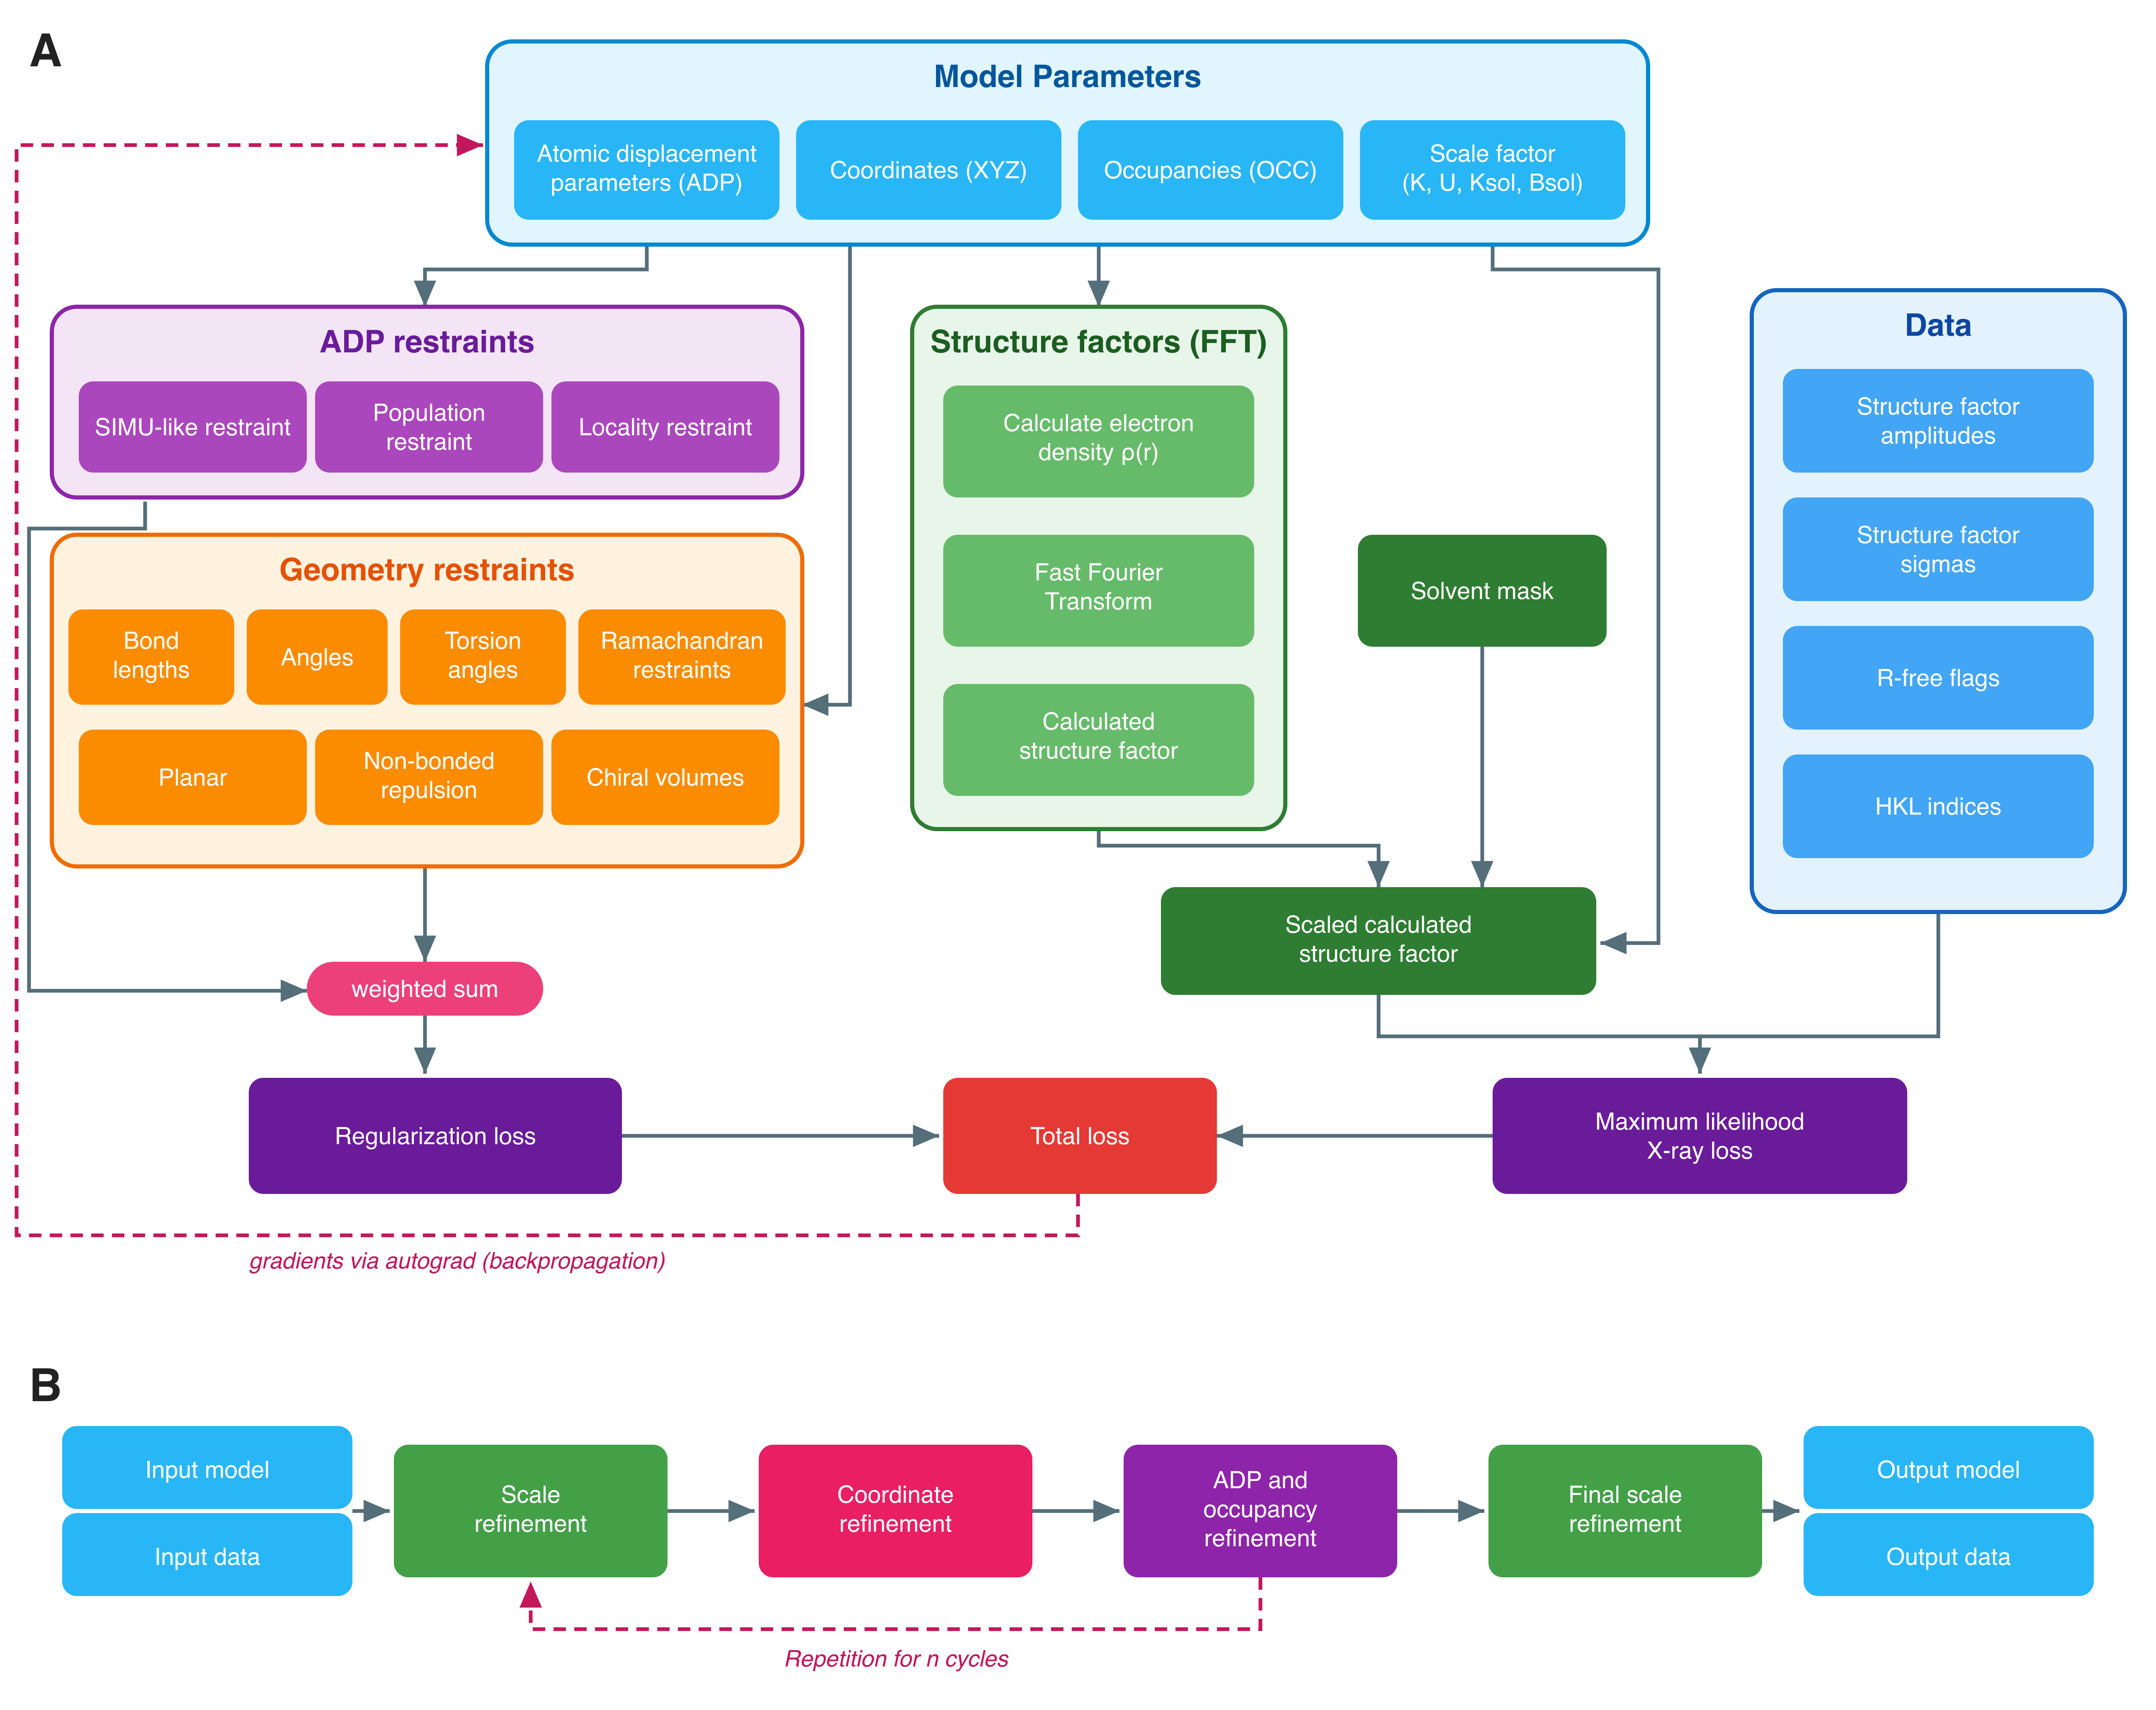
\includegraphics[width=\textwidth]{fig1.png}
\end{center}
\caption{%
  (A) Schematic overview of information flow during a forward pass in the
  standard TorchRef refinement loop.
  The central goal of any macromolecular refinement is to improve the
  data--model fit.
  Atomic coordinates are used to evaluate geometry-based restraint targets:
  bond lengths, bond angles, torsion angles, planarity, non-bonded repulsion,
  chiral volumes, and an opt-in Ramachandran score (off by default and
  unused in the AlphaFold benchmark).
  Atomic displacement parameters are used to feed three regularisation targets:
  a bonded similarity restraint, a shifted inverse-gamma population restraint
  on the $B$-value distribution, and a kNN locality restraint on $\log B$.
  From all model parameters, structure factors $F_\mathrm{calc}$ are computed,
  scaled against experimental data, and compared with observed amplitudes
  $F_\mathrm{obs}$ through a maximum-likelihood target.
  Individual target values are aggregated according to their respective weights
  into a scalar loss, from which gradients are backpropagated to all refinable
  parameters via PyTorch's autograd.
  (B) Overview of the TorchRef refinement workflow.
  The process begins by loading structure coordinates (PDB or mmCIF format) and
  reflection data (MTZ or CIF format).
  An initial scale refinement is performed, followed by the main refinement
  loop: scale update, coordinate refinement, and joint
  optimisation of occupancies and ADPs.
  After the specified number of cycles, a final round of scale refinement is
  performed, followed by writing out the refined model and structure factors.}
\label{fig:fig1}
\end{figure}


%----------------------------------------------------------------------
\subsection{Component weighting}\label{sec:component-weighting}
%----------------------------------------------------------------------

Balancing the X-ray likelihood with geometric restraints and ADP
regularisation is a long-standing challenge in crystallographic refinement.
The default production components are formulated as negative log-likelihoods
or prior penalties on the same loss scale (with least-squares modes retained as
diagnostic alternatives). From first principles these terms can be summed; in
practice, the residual mismatch between the data-fit, geometry, and ADP-prior scales
requires per-group weighting.
TorchRef uses fixed per-group weights
$w_\mathrm{xray} = 1.0$, $w_\mathrm{geometry} = 0.2$, $w_\mathrm{adp} = 0.02$
(\code{DEFAULT_GROUP_WEIGHTS}) as the default; these were calibrated by a
two-dimensional sweep on a subset of the AlphaFold benchmark
(Section~\ref{sec:validation}, Fig.\ S1).
Component-level overrides are exposed at the CLI for users who wish to
fine-tune the weights on a per-structure basis. Adaptive weighting schemes are
planned for future versions of TorchRef (see Discussion).

%----------------------------------------------------------------------
\subsection{Validation of the refinement framework}\label{sec:validation}
%----------------------------------------------------------------------

To verify the functionality of TorchRef, we benchmarked it against \code{phenix.refine} and REFMAC5 under
matched protocols. To create a challenging and realistic test set, we used
AlphaFold predictions placed by molecular replacement and refined them against their respective
experimental datasets.

Starting from a \num{1000}-structure non-redundant set assembled from the
PDB, we mapped each protein chain to its UniProt accession via the Research
Collaboratory for Structural Bioinformatics (RCSB) Data API, downloaded the
corresponding AlphaFold-DB model, and trimmed it to the
crystallised construct.  Residues at which the AlphaFold sequence disagreed
with the construct were truncated to alanine, except at proline and glycine
positions, which were kept as is.  The trimmed search models were
pLDDT$\rightarrow B$-converted with \code{phenix.process_predicted_model}
invoked with \code{maximum_rmsd=100} so that no further
confidence-based residue removal was applied beyond the sequence-based
trimming above; the default pLDDT-to-B mapping of
\code{phenix.process_predicted_model} was used.  The processed models were
placed by Phaser in \code{MR_AUTO} mode using the crystallised composition
\cite{mccoy_phaser_2007}.  Phaser solved \num{767} of \num{825} (\SI{93}{\percent})
AlphaFold-complete structures; the solved subset defines the benchmark set
used.

Placed AlphaFold models were then refined with TorchRef, \code{phenix.refine}
\cite{liebschner_macromolecular_2019}, and REFMAC5 \cite{murshudov_refmac5_2011}
under matched protocols.  All refined models, and the unrefined placed models
for reference, were independently re-scored by \code{phenix.model_vs_data}
against identical structure factors and free flags to produce the R-factors
reported here, holding the scoring conditions constant across engines.
Geometry was assessed by REFMAC5 zero-cycle scoring against a common restraint
library so root-mean-square Z-score (RMSZ) values are comparable across engines.

Of the \num{767} Phaser-solved starting models, Phenix-validated refinements
were obtained for \num{750} with TorchRef, \num{734} with \code{phenix.refine},
and \num{760} with REFMAC5. The dominant failure modes were a special-position
pathology in some Phaser-placed AlphaFold starting models (which is unscoreable
for every engine and additionally caused \code{phenix.refine} to abort), and
out-of-memory (OOM) errors at the 8~GB job limit for TorchRef on the largest
structures (\num{9} structures, all of which pass at 16~GB).
The conserved set on which all three engines refined and Phenix-validated
successfully comprises \num{725} structures; this is the set used for the
headline endpoint comparisons below.

\textbf{R-factors.}
Median Phenix-validated $R_\mathrm{free}$ values were \num{0.3165} for
TorchRef, \num{0.3161} for \code{phenix.refine}, and \num{0.3135} for REFMAC5
(Fig.\ \ref{fig:fig2}A), all substantially below the unrefined prediction's \num{0.4083}.
The three engines therefore agree to within \num{0.30} percentage points, a spread
far smaller than the separation between the refined and unrefined states, so at this
level the differences are of little practical consequence for refinement quality.
Median $R_\mathrm{work}$ values are \num{0.2695} for TorchRef,
\num{0.2719} for REFMAC5 and \num{0.2744} for \code{phenix.refine}: TorchRef reaches
the lowest $R_\mathrm{work}$ but the largest $R_\mathrm{work}$--$R_\mathrm{free}$ gap,
\num{0.0470}, above REFMAC5 (\num{0.0416}) and \code{phenix.refine} (\num{0.0417}).
This gap points to a mild tendency to overfit the working set. 
Broken down per structure, the paired median $R_\mathrm{free}$
difference is $-0.0010$ against \code{phenix.refine} and $+0.0030$ against REFMAC5
(Fig.\ S2). The excess over REFMAC5 is small but statistically robust
($p = 1.6\times10^{-14}$).
TorchRef's internal
$R_\mathrm{free}$ scorer agrees with \code{phenix.model_vs_data} to within
a few tenths of a percentage point, and a cross-scoring analysis on the AlphaFold
benchmark (Fig.\ S3) confirms that no engine favours its own refinement output.
We report Phenix-validated R-factors from \code{phenix.model_vs_data} as a
single external scorer applied uniformly to every engine output.

\textbf{Geometry.}
Bond, angle, chiral, and main-chain $B$-value RMSZ values were computed by REFMAC5
against a uniform restraint library so the metric is comparable across
engines (Fig.\ \ref{fig:fig2}B).
TorchRef's coordinate geometry is essentially on par with REFMAC5: bond, angle, and chiral RMSZ are
\num{0.58}, \num{0.99}, and \num{0.60} for TorchRef, compared with \num{0.58},
\num{0.95}, and \num{0.54} for REFMAC5. This agreement is consistent with both
programs using the CCP4 Monomer Library restraint definitions. The remaining
discrepancy is in the ADPs: TorchRef's main-chain bonded-$B$ RMSZ is \num{1.55},
compared with \num{0.90} for REFMAC5 and \num{1.03} for \code{phenix.refine}. 

\textbf{Weight calibration.}
The default per-group weights were chosen from a two-dimensional sweep of
$(w_\mathrm{geometry}, w_\mathrm{adp})$ at fixed $w_\mathrm{xray} = 1$ on a
subset of the benchmark (Fig.\ S1).
Bond/angle RMSZ tightens as $w_\mathrm{geometry}$ is increased
(Fig.\ S1, top-left), whereas the main-chain bonded-$B$ RMSZ responds primarily
to $w_\mathrm{adp}$ and is treated separately (Fig.\ S1, top-right). Meanwhile,
$R_\mathrm{free}$ shows a U-shaped dependence on $w_\mathrm{geometry}$:
it falls as the geometry weight is increased from very loose values,
reaches a minimum at moderate geometry weights slightly below the chosen
default, and rises sharply once the restraint terms begin to dominate the
X-ray likelihood (Fig.\ S1, bottom-right).
The $R_\mathrm{work}$--$R_\mathrm{free}$ gap closes as either weight is
tightened (Fig.\ S1, bottom-left), so the looser end of the sweep also
carries the heaviest overfitting penalty.
The chosen default $(w_\mathrm{geometry}, w_\mathrm{adp}) = (0.2, 0.02)$
sits just to the tighter side of the $R_\mathrm{free}$ minimum, trading a
small amount of $R_\mathrm{free}$ for tighter bond/angle geometry and a smaller
$R_\mathrm{work}$--$R_\mathrm{free}$ gap.
Pushing the restraint weights further past this point results in significantly worse $R_\mathrm{free}$ values, 
likely due to underfitting and convergence problems; adaptive weighting schemes are planned for a future release.

\textbf{Convergence and runtime.}
Per-cycle program-reported $R_\mathrm{free}$ shows TorchRef and
\code{phenix.refine} converging at essentially the same rate, both reaching
$\sim$\SI{90}{\percent} of their total $R_\mathrm{free}$ improvement by
macrocycle three and both faster in cycle count than REFMAC5
(Fig.\ \ref{fig:fig2}D).  Wall-clock per refinement (Fig.\ \ref{fig:fig2}C)
shows TorchRef \num{4.0} times faster than \code{phenix.refine} but
\num{3.1} times slower than REFMAC5. In a single-core comparison (Fig.\ S4),
TorchRef is \num{21.0} times slower than REFMAC5 and \num{1.4} times slower than
\code{phenix.refine}.
We note that the definition of a macrocycle differs between TorchRef,
\code{phenix.refine}, and REFMAC5, which is reflected in the differing
convergence behaviour. The compiled Fortran implementation of REFMAC5 and its
use of second-derivative information make it more efficient than either
\code{phenix.refine} or TorchRef.

\begin{figure}[ht]
\begin{center}
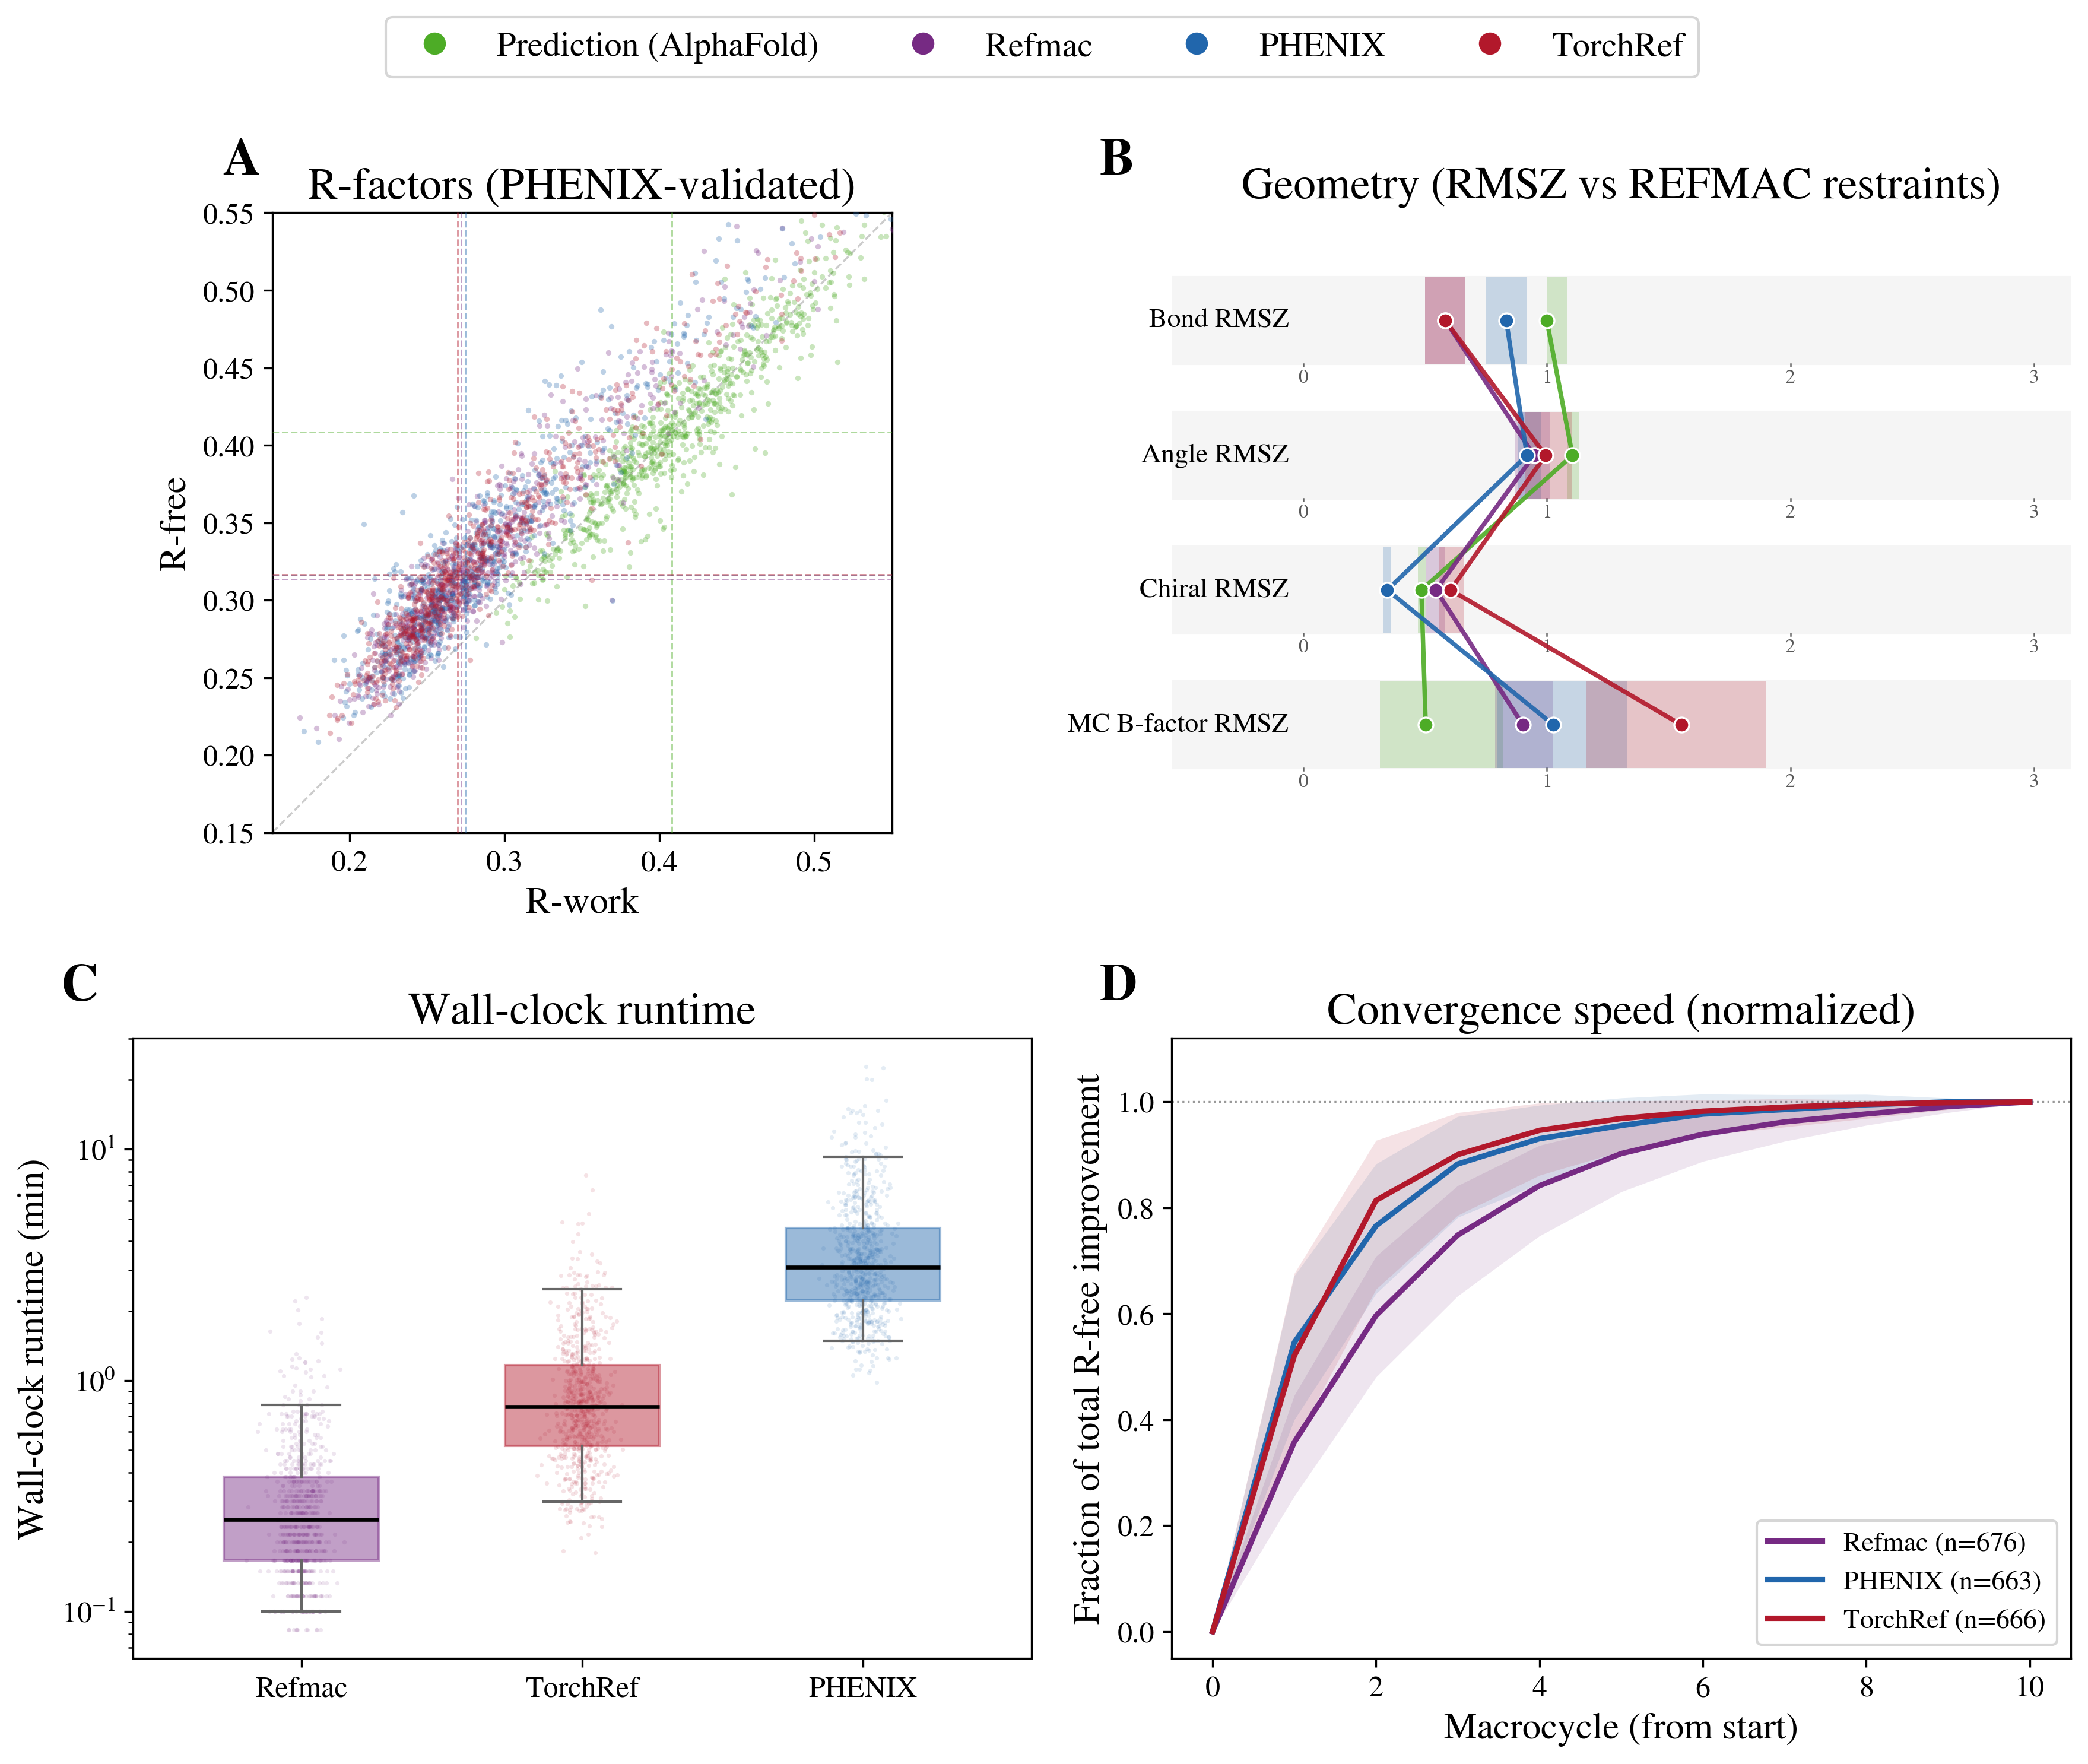
\includegraphics[width=\textwidth]{fig2.png}
\end{center}
\caption{%
  AlphaFold benchmark; \num{767} Phaser-solved candidates. Panels A--C use the
  conserved subset of \num{725} structures on which all three engines refined
  and Phenix-validated successfully. Panel D additionally excludes trajectories
  with less than 0.02 total $R_\mathrm{free}$ improvement, leaving \num{676}
  REFMAC5, \num{663} \texttt{phenix.refine}, and \num{666} TorchRef trajectories.
  R-factors are Phenix-validated under constant scoring conditions; geometry RMSZ
  is REFMAC5-validated against a uniform restraint library.  Engines:
  unrefined AlphaFold prediction (green), REFMAC5 (purple),
  \texttt{phenix.refine} (blue), TorchRef (red).
  (A) $R_\mathrm{free}$ vs $R_\mathrm{work}$ scatter.  Dashed lines mark
  per-engine medians.
  (B) Geometry RMSZ strip (bond, angle, chiral, main-chain $B$-value); point
  $=$ median, band $=$ 25--75\textsuperscript{th} percentile.
  (C) Wall-clock runtime (log scale).
  (D) Convergence speed: fraction of total $R_\mathrm{free}$ improvement vs
  macrocycle, shown as the median across structures with a 25--75\textsuperscript{th}
  percentile band.}
\label{fig:fig2}
\end{figure}


%----------------------------------------------------------------------
\subsection{Performance}
%----------------------------------------------------------------------

TorchRef implements both direct summation-based and FFT-based structure factor
calculations.
Most processes default to the FFT-based structure factor calculation, as it is
more efficient.
This calculation proceeds in three stages.
First, we sample the model's electron density on a real-space grid in P1.
This involves sampling the per-atom electron density on a local grid
(with a per-atom truncation radius based on the ADP and atomic form factor of the atom) 
and then coalescing the local grids onto a
global grid \suppparen{FFT path and electron-density sampling}.
Second, we perform a fast Fourier transform on the grid.
Last, we extract the structure factors from the grid in P1 and apply the
symmetry operations \suppparen{Reciprocal basis and late symmetry expansion}.

Across a set of benchmark structures spanning roughly \num{1300}--\num{10000}
atoms we compare TorchRef's FFT-based structure factor calculation against CCTBX's optimised
routine. We include SFcalculator's direct-summation GPU path \cite{Li2025.01.12.632630} 
in this comparison as it covers similar functionality in enabling structure-factor calculations in a PyTorch framework.
On a single CPU core, TorchRef's FFT-based
forward $F_\mathrm{calc}$ is generally on par with CCTBX's
routine (Fig.\ \ref{fig:fig3}A).
At four cores, TorchRef is generally faster than
CCTBX, with further improvement at sixteen cores.
When running on the GPU (A100) with the custom Triton kernel \cite{tillet_triton_2019},
the forward $F_\mathrm{calc}$ is a median \num{124}-fold faster than CCTBX
(\num{52}--\num{179}-fold across the set; Fig.\ \ref{fig:fig3}A).
For comparison, the direct-summation based structure-factor path of SFcalculator
\cite{Li2025.01.12.632630} running on an A100 is roughly comparable in performance to CCTBX, 
but suffers from out-of-memory errors on the largest two structures (Fig.\ \ref{fig:fig3}A).

A per-target breakdown for pdb\_00001daw of a full refinement iteration shows that the X-ray
target dominates the cost (Fig.\ \ref{fig:fig3}B).
While the classic refinement workload cannot fully exploit the speed of GPU
structure-factor calculations, it does show a significant speedup compared to CPU evaluation.
A complete forward-plus-backward cycle takes $\sim$14~ms on the
GPU and $\sim$75~ms on 8 CPU cores, roughly a five-fold GPU speedup over CPU
evaluation.


\begin{figure}[p]
\begin{center}
  \begin{subfigure}[t]{\textwidth}
    \centering
    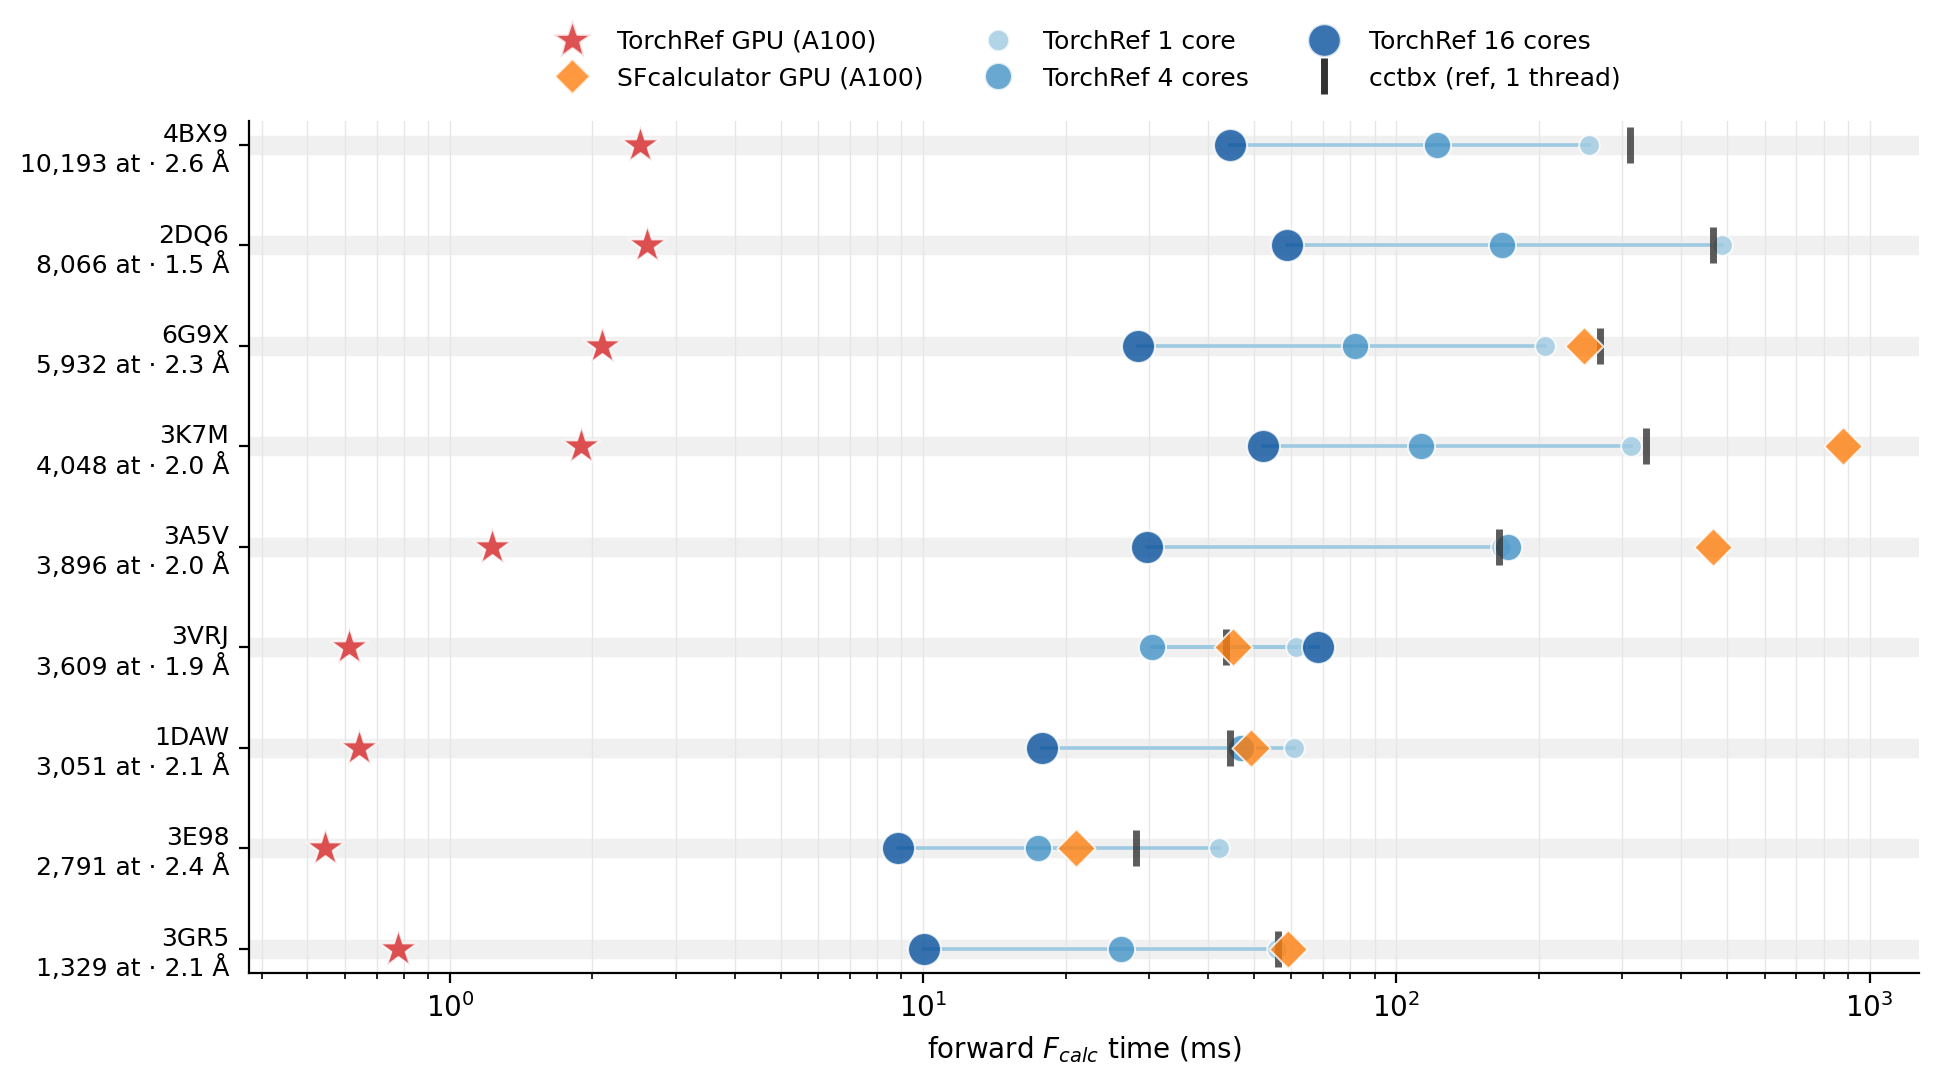
\includegraphics[width=0.85\textwidth]{fig3a.png}
    \caption{}
    \label{fig:fig3a}
  \end{subfigure}\\[1ex]
  \begin{subfigure}[t]{\textwidth}
    \centering
    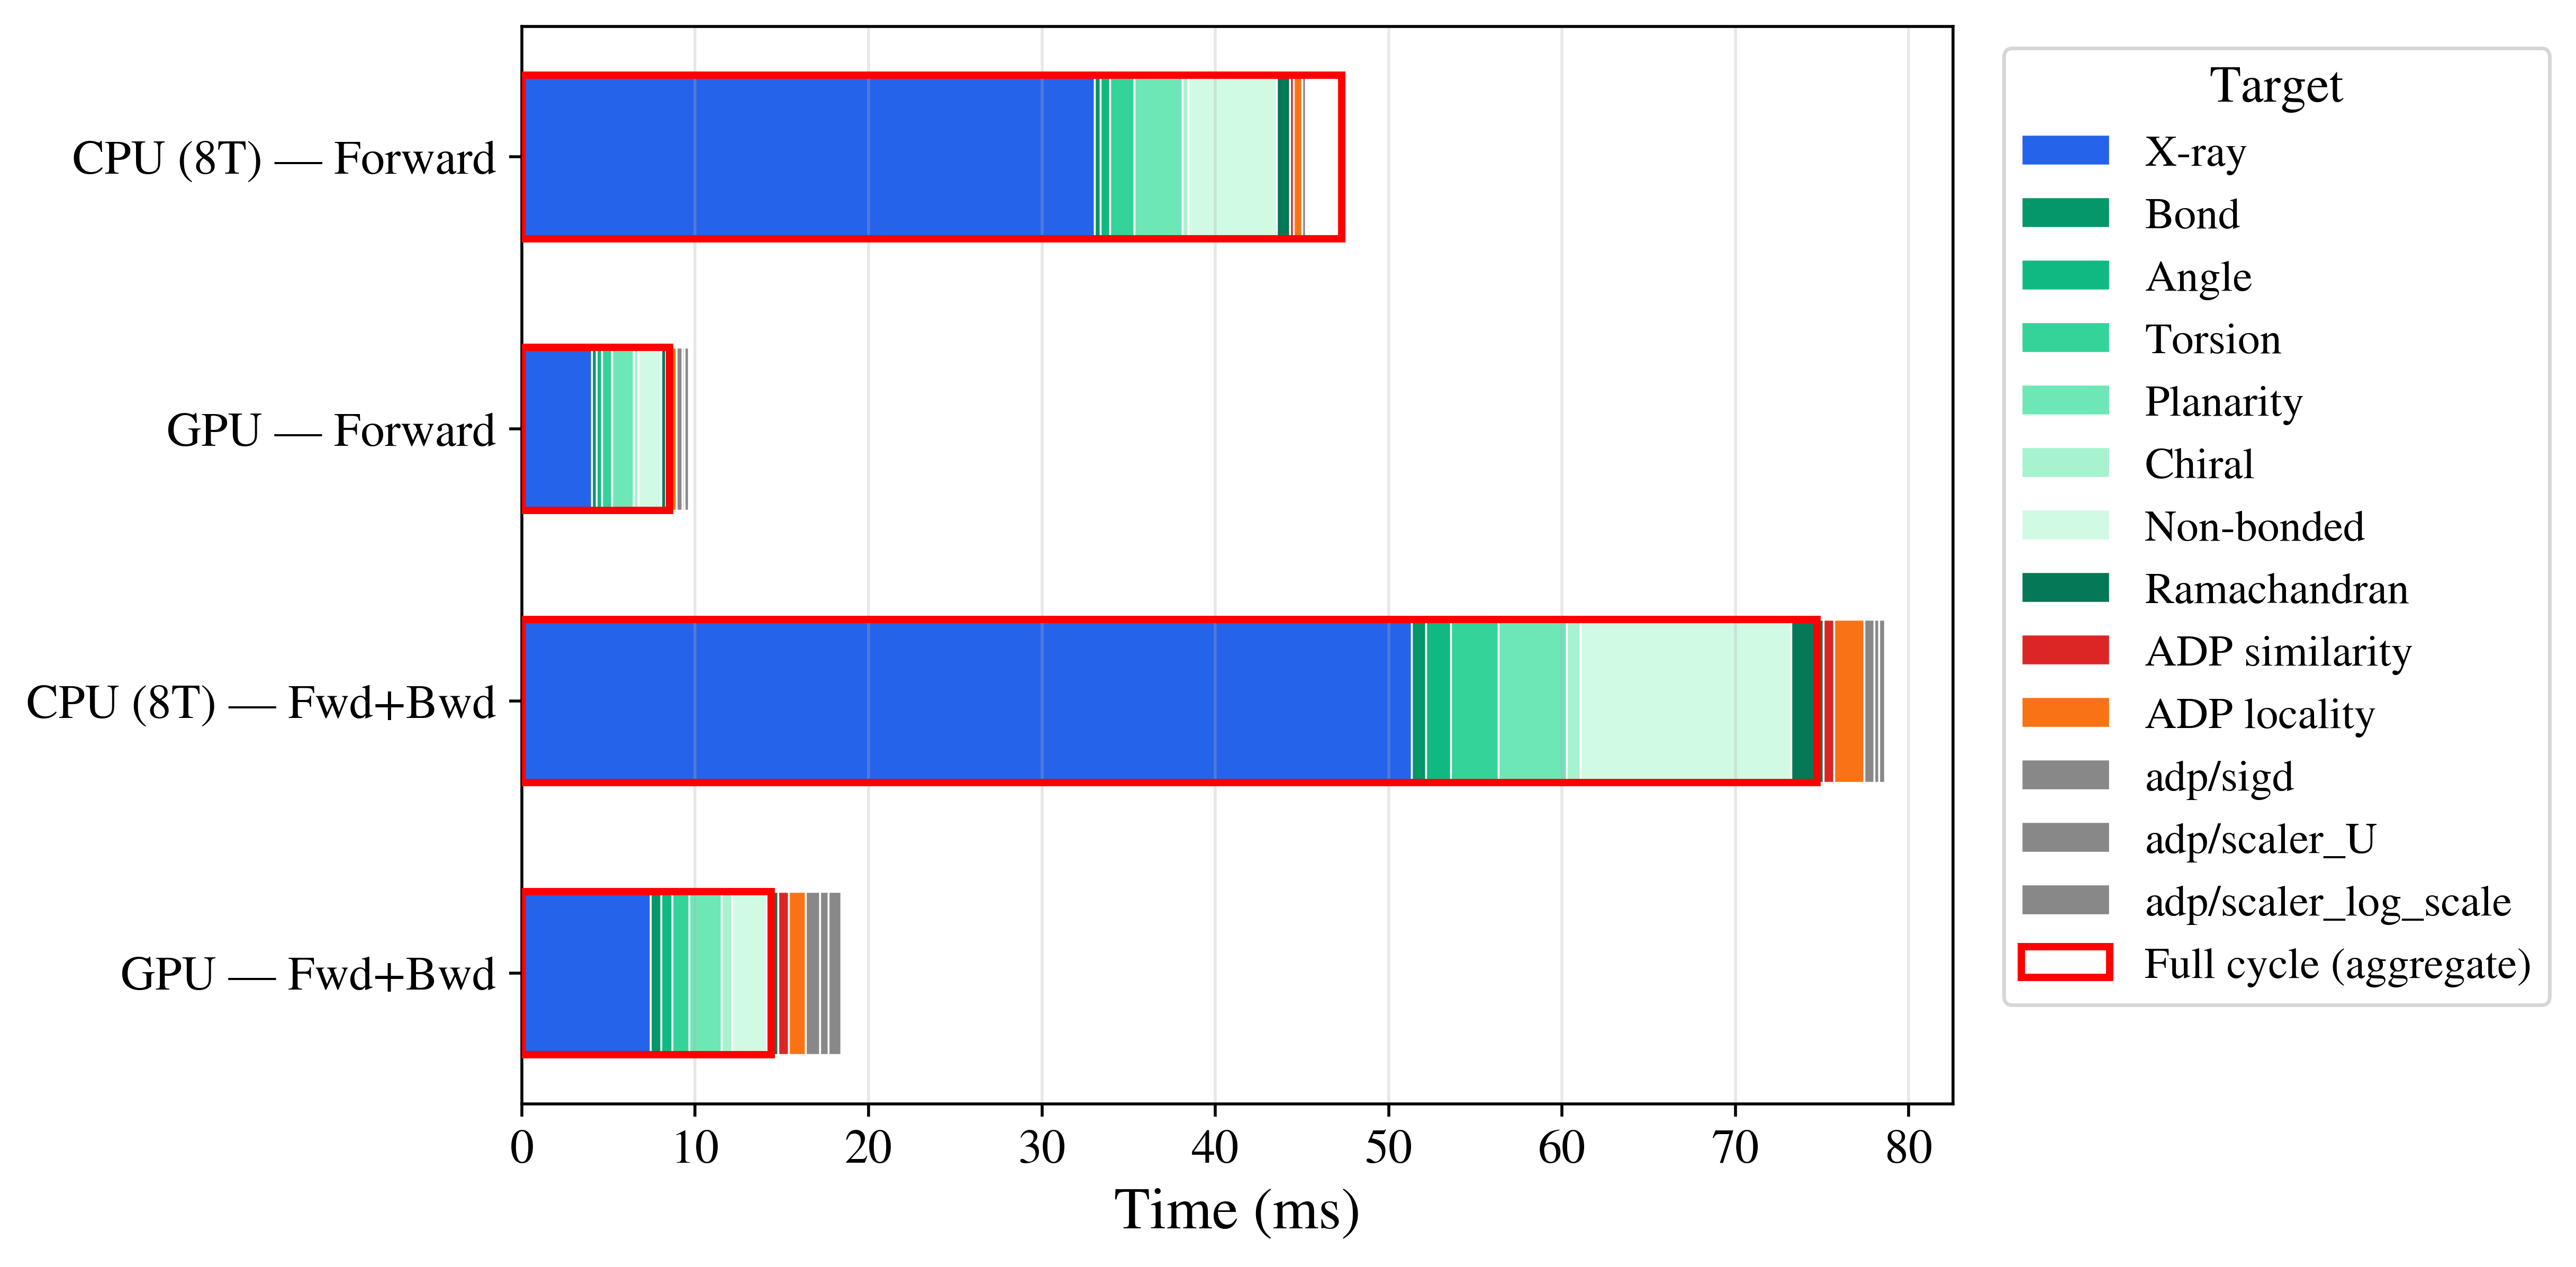
\includegraphics[width=0.85\textwidth]{fig3b.png}
    \caption{}
    \label{fig:fig3b}
  \end{subfigure}
\end{center}
\caption{%
  Structure-factor and refinement-cycle performance.
  GPU timings were recorded on an NVIDIA A100 40~GB; CPU and CCTBX timings on an
  Intel Xeon 6230R (Cascade Lake), chosen to be generation-matched to the A100.
  (A) Forward $F_\mathrm{calc}$ time across nine benchmark structures (one row
  each, labelled by atom count and resolution; log scale), comparing TorchRef on
  the GPU (red stars) and on 1/4/16 CPU cores (light-to-dark blue circles)
  against SFcalculator on the GPU (orange diamonds) and CCTBX on a single CPU
  thread (black ticks, reference).
  TorchRef matches CCTBX on a single core and overtakes it at four cores; on the
  GPU it is a median \num{124}-fold faster than CCTBX (\num{52}--\num{179}-fold
  across the set).
  SFcalculator's direct-summation GPU path is one to two orders of magnitude slower than
  TorchRef's GPU kernel and is absent for the two largest structures, where it
  runs out of memory.
  (B) Per-target time breakdown of a refinement cycle for pdb\_00001daw
  (3,051 atoms, 23,356 reflections, $d_\mathrm{min} = 2.05$~\AA) on CPU (8
  threads) and GPU, for the forward pass and the full forward+backward pass.
  Stacked bars show the individually timed targets: the X-ray target
  dominates, and the hollow red box is the independently measured full cycle.
  A full forward+backward cycle takes $\sim$14~ms on the GPU and $\sim$75~ms on
  8 CPU cores.}
\label{fig:fig3}
\end{figure}


%----------------------------------------------------------------------
\subsection{Difference refinement}
%----------------------------------------------------------------------

The end-to-end differentiability of TorchRef enables gradient propagation
through complex computational pipelines that would be difficult to implement in
conventional refinement programs.
In particular, it supports multi-model, multi-dataset workflows.
As an example, we implement difference-amplitude-based refinement
\cite{berendzen_difference_1995}, which is useful for time-resolved
crystallography and related fields.
Alongside the geometric restraints and atomic-displacement regularisation
already in the refinement, we add an X-ray difference loss: a Gaussian negative
log-likelihood on the amplitude differences between two related datasets
(a Gaussian negative log-likelihood is, up to additive constants independent of
the refined parameters, equivalent to an inverse-variance-weighted
least-squares residual).
Because the target models the difference directly, systematic errors common to 
both datasets cancel rather than bias the fit. We further place a
spike-and-slab prior on the per-atom coordinate change between the dark and light models, 
treating small displacements as noise (the spike) while leaving larger, genuine movements 
essentially unpenalised (the slab). The full target, the mixed-model parameterisation, and 
the prior are derived in \suppref{Difference refinement for time-resolved data}.

Combining this with mixed-model refinement, where we define a combined model as
a linear combination of a reference and a light model, we can optimise the
light model to explain the observed structure factor differences.
This is a simple example of a multi-model, multi-dataset approach that can be
extended to fit the data \suppparen{Multi-dataset and multi-model infrastructure}.

To validate different solutions, we implemented a command-line tool that
calculates local correlation coefficients between the weighted difference
observed structure factor (WDF$_\mathrm{o}$) density map and the weighted
difference calculated structure factor (WDF$_\mathrm{c}$) density map for a
given atom selection and masking radius (see Materials and Methods) under
consideration of the dark phases.
Here, we use inverse-variance weights for the difference observations.
Additionally, we calculate reciprocal-space correlation on the differences.
Localisation of the signal within the structure yields noticeably higher
real-space correlations than reciprocal-space correlations, allowing
meaningful correlations to be extracted even for a strongly localised
change.

To assess the utility of the difference-refinement approach, we applied it to
dataset pdb\_00007yyz from a time-resolved serial crystallography study of the
photo-pharmacological drug azo-combretastatin A4 (azo-CA4) bound to
$\alpha\beta$-tubulin \cite{wranik_watching_2023} (for the full refinement
protocol, see Materials and Methods).
In that study, cis-to-trans photoisomerisation of the azobenzene moiety was
triggered by light, and nine structural snapshots spanning 1~ns to 100~ms
captured the resulting ligand release and collapse of the colchicine-site
binding pocket.
The pdb\_00007yyz dataset corresponds to the 10~$\mu$s timepoint, at which the ligand
has begun to shift but remains bound.
The deposited structure was originally refined with \code{phenix.refine} using extrapolated
structure factors at an estimated light-state occupancy of 0.22.

TorchRef difference refinement was performed with a resolution cutoff of
2.2~\AA{} at an assumed light-state occupancy of 0.22, matching the published
structure. The occupancy can optionally be refined, but from a single timepoint
this is generally not recommended and any refined value must be interpreted with
care, so we fixed it to the published estimate.
Within a 2.5~\AA{} radius around both the dark and light conformations of the
IBL ligand (azo-CA4), the resulting model matched the WDF$_\mathrm{o}$ with a
local correlation of 0.85, compared to 0.74 for the deposited model refined
using extrapolated structure factors (Fig.\ \ref{fig:fig4}).
Considering the global fit of the model, the calculated difference structure
factor amplitudes show correlations of 0.51 and 0.31 with the observed
difference structure factor amplitudes for the TorchRef difference-refined
model and the extrapolated model, respectively.
Notably, the differences in the resulting structures are subtle and the models
are qualitatively similar.

\begin{figure}[ht]
\begin{center}
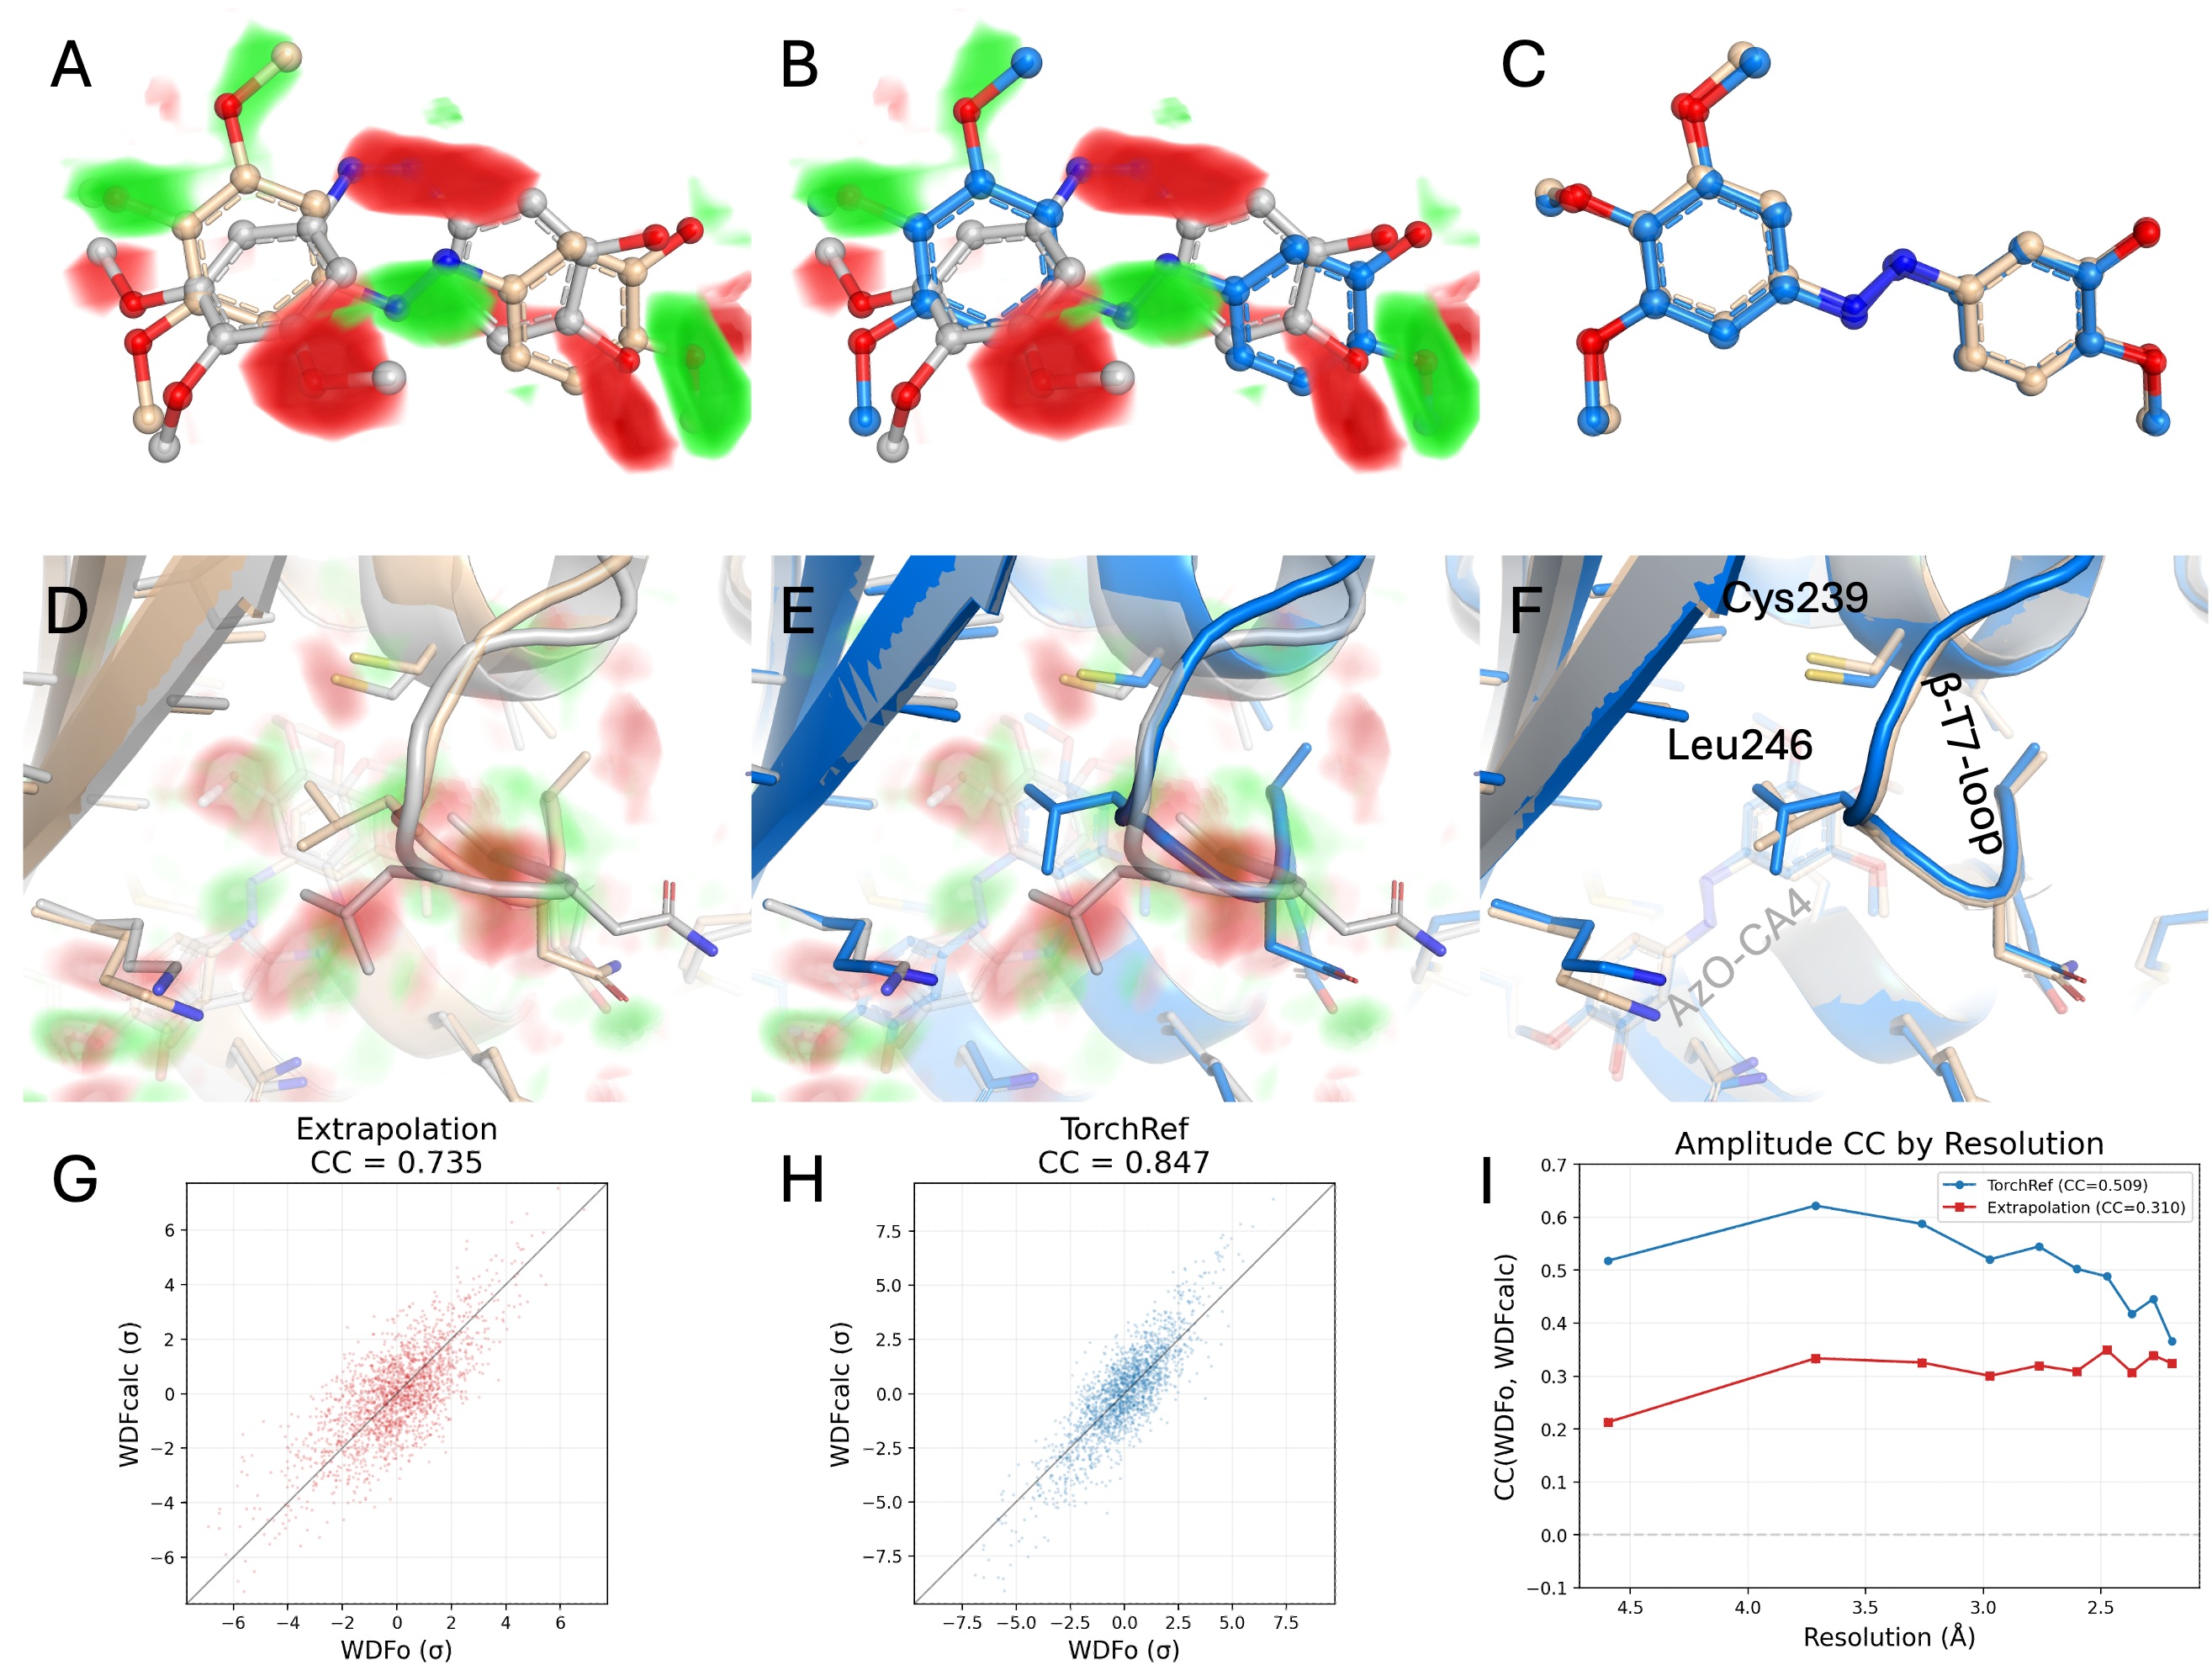
\includegraphics[width=\textwidth]{fig4.png}
\end{center}
\caption{%
  Difference refinement of azo-CA4 (IBL) \emph{cis}-to-\emph{trans}
  isomerisation in tubulin (pdb\_00007yyz).
  Weighted difference electron density (WDF$_\mathrm{o}$) maps are visualised
  via a volume ramp from 3 to 5~$\sigma$ around the ligand (green, positive;
  red, negative) (A, B) and 2.5 to 4.5~$\sigma$ in the wider binding pocket
  (D, E).
  Top row (A--C): IBL ligand close-up.
  Bottom row (D--F): binding pocket view showing the changes in the
  $\beta$t7-loop resulting from the unbinding of the \emph{trans} conformer
  ligand.
  Dark-state structure pdb\_00008ql2 (grey), published extrapolated structure pdb\_00007yyz
  (wheat), and TorchRef difference-refined structure (blue).
  (A, D) WDF$_\mathrm{o}$ map with the deposited pdb\_00007yyz structure refined from
  extrapolated structure factors.
  (B, E) WDF$_\mathrm{o}$ map with the TorchRef difference-refined structure.
  (C, F) Superposition of the TorchRef-refined (blue) and deposited pdb\_00007yyz
  (wheat) conformations, showing the agreement and differences between the
  independently determined light-state structures.
  Scatter plots G and H show the distribution of WDF$_\mathrm{c}$ voxel values
  relative to WDF$_\mathrm{o}$ voxels within a 2.5~\AA{} radius around the dark
  and light conformations of the ligand.
  G shows the scatter plot for the extrapolated data, while H shows the
  TorchRef difference-refinement scatter plot.
  The correlation between calculated and observed difference amplitudes is
  shown in panel I, binned by resolution.}
\label{fig:fig4}
\end{figure}


%==============================================================================
\section{Discussion}
%==============================================================================

TorchRef provides a PyTorch-based crystallographic refinement framework that
exposes all relevant parameters to automatic differentiation.
This design paradigm offers significant advantages over classic
implementations, as it correctly handles complex gradient computations through
automatic backpropagation, removing the need for manually derived analytical
gradients.
This not only reduces implementation effort but also eliminates an important
source of programming errors when developing new refinement targets or
parameterisations.
TorchRef's native PyTorch implementation enables deep integration with the
growing ecosystem of PyTorch-based tools in structural biology, including
molecular dynamics engines such as TorchMD \cite{doerr_torchmd_2021},
structural prediction models such as OpenFold \cite{ahdritz_openfold_2024} (as demonstrated by the recent Rocket project \cite{fadini_alphafold_2026}), and
machine-learning-accelerated quantum-mechanical potentials such as those used
in AQuaRef \cite{zubatyuk_aquaref_2025}.

A central concern for any new refinement framework is whether its design
choices compromise refinement quality. Across 725 Phaser-placed
AlphaFold predictions refined head-to-head with \code{phenix.refine},
REFMAC5, and TorchRef, the three engines reach median $R_\mathrm{free}$ values
within 0.30 percentage points of each other
(TorchRef \num{0.3165}, \code{phenix.refine} \num{0.3161}, REFMAC5 \num{0.3135}),
a spread small enough that the differences carry no practical weight, even though
the paired comparison against REFMAC5 remains statistically resolvable in its favour.
TorchRef reaches the lowest median $R_\mathrm{work}$ but the largest
$R_\mathrm{work}$--$R_\mathrm{free}$ gap (\num{0.0470}, against
\num{0.0416}--\num{0.0417} for the reference engines), a mild overfitting
signature.  We hypothesise that the current global fixed-weight target contributes
to it and that resolution-dependent or adaptive weighting would reduce it, though the
concurrent tendency towards low absolute ADPs (main-chain bonded-$B$ RMSZ \num{1.55}
against \num{0.90} for REFMAC5) leaves open an ADP-driven component.  TorchRef's
coordinate-geometry RMSZ is essentially on par with REFMAC5, consistent with the
use of the same CCP4 monomer-library restraint definitions.  The one clear
residual is a small $R_\mathrm{free}$ excess relative to REFMAC5 (paired median
$+0.0030$), whereas against \code{phenix.refine} TorchRef is marginally lower.


The difference-refinement procedure demonstrates a use case that is difficult
to implement in conventional refinement programs.
Existing approaches to time-resolved crystallographic data analysis typically
rely on extrapolated structure factors, which amplify the signal from a partially
occupied excited state to simulate a fully occupied one.
While powerful, extrapolation introduces noise amplification that scales
inversely with occupancy.

Additionally, because extrapolated structure factor amplitudes are calculated
with phases derived from the dark state, any phase difference between the dark
and light models introduces error into the resulting maps.
Extrapolation also systematically produces negative amplitudes from phase
mismatches and noise amplification.
The standard correction protocols absorb this as additional noise in the
active region rather than as a systematic bias, which accounts for the
general success of extrapolation-based methods while leaving the
excited-state density noisier than the true signal.
Modern extrapolation tools further apply Bayesian weighting that downweights
noisy-difference amplitudes, at the cost of shrinking the signal toward
the dark reference \cite{de_zitter_xtrapol8_2022}.

Direct refinement of a mixed model against amplitude differences, as
implemented in TorchRef, sidesteps these issues by fitting the difference
between the dark-state model and the occupancy-weighted combination of dark- and
light-state models to the observed difference in the dark and light data.
In the case of pdb\_00007yyz, this approach yielded a higher local correlation between
calculated and observed difference maps (0.85 vs 0.74 for the deposited
structure around the chromophore).
The differences between the extrapolated structure and the
TorchRef-difference-refined structure are subtle, but the local-correlation
improvement is reproduced across the chromophore region.
Beyond the two-dataset case shown here, this approach extends naturally to
more than two datasets and multiple transient structures.

TorchRef is designed as a platform for method development and does not yet
implement the full feature set of established refinement packages.  On the
modelling side, it lacks automated water placement and deletion,
non-crystallographic symmetry (NCS) restraints, reference-model restraints,
twinning support, and translation--libration--screw (TLS) parameterisation.  On
the optimisation
side, simulated annealing and Langevin-style stochastic optimisers are implemented
as experimental alternatives, but they are not part of the production protocol
benchmarked here and still require systematic validation. On the target side,
adaptive weighting remains an open problem and may help reduce the small
residual $R_\mathrm{free}$ excess. Qualitative inspection of the rerun models
shows a systematic tendency towards low absolute ADPs, pointing to a possible
scale-factor--ADP interaction; this diagnosis is provisional and will be tested
in future work.

Looking ahead, TorchRef's modular architecture opens several avenues for
development.
The multi-model, multi-dataset framework demonstrated here for difference
refinement generalises naturally to kinetic multi-state refinement against
time-resolved serial crystallography data, where a small number of
conformational states would be refined against many datasets simultaneously.
As an experimental proof of concept for force-field integration, TorchRef
already includes a working differentiable AMBER14/GAFF2 target
\cite{maier_ff14sb_2015,wang_gaff_2004} coupled to OpenMM
\cite{eastman_openmm_2017}, with analytical forces bridged into PyTorch
autograd, non-standard residues parameterised on the fly via antechamber
\cite{wang_antechamber_2006}, and a riding-hydrogen model that redistributes H
forces onto the heavy-atom frame. The AMBER target is not yet at production
quality and is not used in the AlphaFold benchmark above.
Replacing the empirical AMBER potential with learned energy surfaces such as
MACE-OFF \cite{kovacs_mace-off_2025} or AIMNet2 \cite{anstine_aimnet2_2025}
would combine deep-learned physical priors with the data-driven X-ray maximum
likelihood, much as AQuaRef \cite{zubatyuk_aquaref_2025} has demonstrated for
quantum-mechanical refinement within Phenix, but with the advantage that, in
TorchRef, the potential is a native PyTorch module and its gradients propagate
through the same computational graph as the other targets of the refinement.

Given the well-documented, open-source nature of TorchRef, we hope to make the
development of custom refinement protocols accessible to a broader community of
crystallographers and method developers.
The full API documentation, Jupyter notebook tutorials, and permissive MIT
license are intended to lower the barrier to experimentation.
As a concrete example, the difference refinement was initially implemented in
approximately \num{1000} lines of Python code (of which the core logic accounts for \num{200} lines), a
task that would require substantially more effort in a conventional refinement
codebase, where analytical gradients must be derived and implemented by hand.

We hope that TorchRef, or projects like it, will allow many more researchers to contribute effectively
to macromolecular structure refinement, a field in which the depth and complexity of established
codebases have historically concentrated methodological development among a small number of
specialists. We are open to contributions and collaborations, and welcome feedback to help shape the future of TorchRef.


%==============================================================================
\section{Materials and Methods}
%==============================================================================

%----------------------------------------------------------------------
\subsection{Structure selection and dataset preparation}
%----------------------------------------------------------------------

A non-redundant benchmark dataset of \num{1000} protein crystal structures was
assembled from the Protein Data Bank (PDB).
Structures were selected programmatically via the RCSB PDB Search API using the
following criteria:
(i) experimental method restricted to X-ray diffraction,
(ii) resolution between 1.5 and 3.0~\AA{}, and
(iii) maximum pairwise sequence identity of 30\%, enforced by retaining only
cluster representatives from the RCSB sequence clustering at the 30\% identity
level.
From an initial pool of \num{1500} candidate entries, structures were filtered to
retain only those with deposited structure factor data, yielding the final set
of \num{1000} structures.
For each structure, coordinate files (PDB and macromolecular CIF (mmCIF)
formats) and structure factor files (structure factor CIF (SF-CIF) format)
were downloaded from the RCSB.


%----------------------------------------------------------------------
\subsection{MTZ conversion and R-free flag generation}
%----------------------------------------------------------------------

Structure factor CIF files were converted to MTZ format using TorchRef's
ReflectionData module.
$R_\mathrm{free}$ flags were regenerated for all structures
(\code{regenerate_rfree_flags(force=True)}), as deposited flags were
inconsistent across the benchmark set.
Flags are assigned by resolution-stratified random sampling: the reflections
are binned in shells of $d^{*2}$ and a fixed fraction of each shell is drawn at
random. Reflections are stored in the canonical CCP4 asymmetric unit, so every
space-group-symmetry equivalent maps to a single ASU reflection and shares its
flag. The generator does not, however, currently group reflections related by
higher \emph{metric} (lattice) symmetry (for example twin operators or
pseudosymmetry not expressed by the space group), so under twinning or
pseudosymmetry a free reflection could be related to a working reflection,
leaking information across the work/free boundary; metric-symmetry-aware flag
grouping is planned as future work. We did not perform a dedicated cohort-wide
twinning or pseudosymmetry screen and therefore do not claim that these
pathologies are absent from every benchmark structure.

%----------------------------------------------------------------------
\subsection{AlphaFold search model preparation and molecular replacement}
%----------------------------------------------------------------------

For each benchmark structure, each protein chain was mapped to its UniProt
accession via the RCSB Data API (GraphQL endpoint), and the corresponding
AlphaFold2 model was downloaded from the AlphaFold DB
(\code{alphafold.ebi.ac.uk/api/prediction/{accession}}).
Structures for which every protein chain had an AlphaFold model
(\code{af_complete}) defined the AlphaFold benchmark cohort.

Per UniProt component, the AlphaFold model was aligned to the crystallised
construct sequence using \emph{gemmi} pairwise alignment
\cite{wojdyr_gemmi_2022}.
From the alignment: (i) AF-only flanks and insertions were trimmed;
(ii) residues matching the construct were retained;
(iii) residues whose AlphaFold identity disagreed with the construct were
truncated to alanine (residue renamed ALA, side chain stripped to
\{N, C$\alpha$, C, O, C$\beta$\}), except proline and glycine, which were
kept as is.
Trimmed search models were then pLDDT$\rightarrow B$-converted with
\code{phenix.process_predicted_model} (\code{maximum_rmsd=100}, disabling
confidence-based residue removal since the model was already trimmed) and
placed by \code{phenix.phaser} in \code{MR_AUTO} mode using the crystallised
composition (\code{ENSEMBLE ... IDENTITY 0.9}; one
\code{SEARCH ENSEMBLE ... NUMBER {copies}} per UniProt component).
The top Phaser solution was retained as the placed search model.
Out of \num{825} AlphaFold-complete entries, Phaser produced a solution for \num{767}
structures (\num{93}\%), defining the benchmark arm used here.
The \num{58} structures that failed Phaser MR were excluded.

%----------------------------------------------------------------------
\subsection{Refinement protocols}
%----------------------------------------------------------------------

The placed AlphaFold model was refined against the structure factors by each
engine in turn, using matched protocols and identical hardware (Slurm-managed
cluster, four CPU cores and 8~GB of RAM per job):

\textbf{TorchRef:} \code{torchref.refine} (v0.6.4), 10 macrocycles, alternating
coordinate, ADP/occupancy, and scaler blocks (\code{--mode separate}); the
default $\sigma_{A}$ maximum-likelihood X-ray target (\code{--xray-mode ml})
and default group weights $w_\mathrm{xray}=1.0$, $w_\mathrm{geometry}=0.2$,
$w_\mathrm{adp}=0.02$.

\textbf{Phenix:} \code{phenix.refine} v1.20-4459 \cite{liebschner_macromolecular_2019},
10 macrocycles with the \code{individual_sites + individual_adp + occupancies}
strategy (separate refinement of atomic coordinates, individual isotropic
$B$-values, and partial occupancies), bulk-solvent and overall scaling enabled,
ordered solvent disabled, Ramachandran restraints enabled, simulated annealing
and target-weight optimisation disabled.

\textbf{REFMAC5:} \code{refmac5} from the CCP4 suite v7.1
\cite{murshudov_refmac5_2011, agirre_ccp4_2023}, 10 NCYCLES restrained
refinement, \code{MAKE HYDR NO}, with \code{FreeR_flag} read from the input
MTZ.

%----------------------------------------------------------------------
\subsection{R-factor scoring and cross-scorer validation}
%----------------------------------------------------------------------

All refined models, and the unrefined placed search models for reference, were
independently re-scored against identical structure factors and free flags by
three R-factor scorers operating in zero-cycle mode (scaling and bulk-solvent
fit only; coordinates and ADPs untouched):
REFMAC5 with \code{NCYCLES 0} \cite{murshudov_refmac5_2011};
\code{phenix.model_vs_data} \cite{liebschner_macromolecular_2019};
and \code{torchref.refine -n 0} on the same model.
For the main figure, \code{phenix.model_vs_data} provides the headline
R-factors. Geometry RMSZ values reported in Fig.\ \ref{fig:fig2}B were computed from the
REFMAC5 zero-cycle restraint table so the underlying restraint library is
uniform across engines.
Wall-clock per refinement was taken from each program's own log files for
successful runs.

%----------------------------------------------------------------------
\subsection{Benchmarking structure factor calculation and gradient performance}
%----------------------------------------------------------------------

\subsubsection{Test system}

The forward $F_\mathrm{calc}$ scaling benchmark (Fig.\ \ref{fig:fig3}A) used a
set of nine structures spanning roughly \num{1300}--\num{10000} atoms and
resolutions of \num{1.5}--\num{2.6}~\AA{}.
The per-target refinement-cycle breakdown (Fig.\ \ref{fig:fig3}B) used the
crystal structure pdb\_00001daw, comprising \num{3051} atoms and \num{23356}
unique reflections at a resolution of 2.05~\AA{}.

\subsubsection{Quantities benchmarked}

Three timing scenarios were measured for TorchRef, each calling
\code{compute_structure_factors} directly (bypassing the model cache):

(1)~\textbf{Forward:}
Structure factor calculation $F_\mathrm{calc}(\mathbf{h})$ inside a
\code{torch.no_grad} context, measuring the raw forward-pass cost without
constructing a computational graph.

(2)~\textbf{Backward only:}
A forward pass followed by \code{loss.backward()} (where
loss = $\sum |F_\mathrm{calc}|$), with only the backward pass timed.
This isolates the cost of automatic differentiation through the structure
factor kernel.
This timing is less accurate than combined forward+backward pass evaluations
due to timing overhead.

(3)~\textbf{Forward + backward:}
End-to-end $F_\mathrm{calc}$ computation plus gradient back-propagation, timed
together.

As a reference, the forward-only $F_\mathrm{calc}$ computation via CCTBX
(\code{xray_structure.structure_factors(d_min=...).f_calc()}) was timed on
CPU under identical conditions, using
\code{cctbx-base} (the version pinned by the TorchRef installation) and
the same \code{OMP_NUM_THREADS}/\code{MKL_NUM_THREADS}/%
\code{OPENBLAS_NUM_THREADS} caps as the TorchRef runs.
CCTBX gradients were not benchmarked: a documented public API for
differentiating \code{f_calc()} through CCTBX was not identified at the
time of writing.
As a second reference, SFcalculator \cite{Li2025.01.12.632630} was benchmarked
on the GPU for the forward $F_\mathrm{calc}$ under matching conditions;
out-of-memory failures on the largest structures were recorded as such.

\subsubsection{CPU thread scaling}

To assess parallelism, benchmarks were run across 1--16 CPU threads; the
$F_\mathrm{calc}$ scaling figure reports 1, 4, and 16 cores.
Each configuration was executed in an isolated subprocess with
\code{TORCHREF_NUM_THREADS}, \code{OMP_NUM_THREADS},
\code{MKL_NUM_THREADS}, and \code{OPENBLAS_NUM_THREADS} all set to the
target thread count, ensuring consistent control over intra-op parallelism in
PyTorch, BLAS, and OpenMP.
The TorchRef \code{__init__} module reads \code{TORCHREF_NUM_THREADS}
and calls \code{torch.set_num_threads()} accordingly.

\subsubsection{GPU benchmarks}

GPU timings were collected on an NVIDIA A100-PCIE-40~GB.
All GPU timings bracket each iteration with \code{torch.cuda.synchronize()}
to ensure asynchronous kernel launches are fully completed before reading the
wall-clock time.

\subsubsection{Timing protocol}

For each configuration (thread count and device), three warm-up iterations
were run followed by 10 timed iterations.
Wall-clock time was measured with \code{time.perf_counter()}.
Summary statistics reported are the mean, minimum, and maximum over the 10
timed iterations.
Speedup is defined as the ratio of the single-thread CPU mean time to the mean
time at a given thread count (or on GPU).

\subsubsection{Loss function timing}

Loss function timings used TorchRef's default loss function initialisation, as
in a standard refinement setup.
We then evaluated the forward and backward passes for the loss functions commonly used in refinement.

%----------------------------------------------------------------------
\subsection{Difference refinement}
%----------------------------------------------------------------------

Difference refinement was performed with \code{torchref.difference-refine},
which targets the residual between the observed and calculated structure
factor amplitude differences of the light and dark datasets,
with the dark model held fixed \suppref{Difference refinement for time-resolved data}.
Refined models were validated with \code{torchref.validate-ded}, which reports
the local correlation between the weighted observed difference map
($\mathrm{WDF}_o$, from $F_\mathrm{obs}^\mathrm{light} - F_\mathrm{obs}^\mathrm{dark}$)
and the weighted calculated difference map
($\mathrm{WDF}_c$, from $|F_\mathrm{calc}^\mathrm{mix}| - |F_\mathrm{calc}^\mathrm{dark}|$)
within a masking radius around a selected atom set; maps were calculated using
dark-state phases and Bayesian weights.

To demonstrate the approach we refined against PDB entry pdb\_00007yyz
\cite{wranik_watching_2023}, a time-resolved serial crystallography structure of
a photoisomerised azobenzene-analogue ligand.  The deposited model was originally
refined with \code{phenix.refine} using extrapolated structure factors at 0.22 occupancy and a
2.2~\AA{} resolution cutoff.  For TorchRef difference refinement we used the
recently released dark structure pdb\_00008ql2 as both the initial light and
dark model with a fixed 22\% light-state fraction.  Following an automated
pass, two cycles of manual real-space adjustment in Coot, using the
phase-corrected extrapolated structure factors written by
\code{torchref.difference-refine}, alternated with refinement; a final
equilibration cycle set both the difference-target and coordinate-similarity
weights to 1.  Reflections were used to 2.2~\AA{}, validation correlations were
computed at the same resolution to allow direct comparison with the deposited
model, and $R_\mathrm{free}$ flags were grafted from the pdb\_00008ql2 dataset
to give meaningful $R_\mathrm{free}$ values.


%==============================================================================
\section{Data and Code Availability}
%==============================================================================

TorchRef is available on GitHub under an MIT license and can be installed via
pip.
Full API documentation and Jupyter notebook tutorials are available via GitHub
at github.com/HatPdotS/TorchRef.
The scripts used to generate the figures are available via GitHub.
The difference-refined structure is pending release in the PDB and will be
available under code pdb\_0000030as.


%==============================================================================
% Back matter
%==============================================================================

\begin{acknowledgements}
The project was conceived by H.-P.S. and T.W.
The code was authored by H.-P.S. under the supervision of T.W. and J.S.
The manuscript was authored by H.-P.S. and T.W. with input from J.S.
Figures were made by H.-P.S. with the help of T.W.
The manuscript was reviewed by J.S., T.W. and H.-P.S.
Claude Code was used during the development of TorchRef for
prototyping, refactoring, and documentation.
Claude was used to review and rephrase text during the preparation of this
manuscript.
\end{acknowledgements}

\begin{funding}
This work was supported by Swiss National Science Foundation project grants
10.007.643 (J.S.) and 10.003.847 (T.W.).
\end{funding}

\ConflictsOfInterest{The authors declare that they have no conflicts of
  interest.}

\DataAvailability{TorchRef is available on GitHub at
  github.com/HatPdotS/TorchRef under an MIT license.
  All benchmark data and scripts are available in the repository.
  The difference-refined structure is pending release in the PDB and will be
  available under code pdb\_0000030as.}


\bibliography{torchref}


\end{document}
